% Empirical Comparison of Memory Architectures for Bias-Resistant Multi-Agent LLM Systems
% TMLR Submission — official JmlrOrg/tmlr-style-file template
% https://github.com/JmlrOrg/tmlr-style-file/blob/main/main.tex

\documentclass[11pt]{article}
\usepackage[preprint]{tmlr}
% If accepted, switch to: \usepackage[accepted]{tmlr}

%%%%% NEW MATH DEFINITIONS %%%%%
%%%%% From JmlrOrg/tmlr-style-file/main
%%%%% https://github.com/JmlrOrg/tmlr-style-file/blob/main/math_commands.tex

\usepackage{amsmath,amsfonts,bm}

% Mark sections of captions for referring to divisions of figures
\newcommand{\figleft}{{\em (Left)}}
\newcommand{\figcenter}{{\em (Center)}}
\newcommand{\figright}{{\em (Right)}}
\newcommand{\figtop}{{\em (Top)}}
\newcommand{\figbottom}{{\em (Bottom)}}
\newcommand{\captiona}{{\em (a)}}
\newcommand{\captionb}{{\em (b)}}
\newcommand{\captionc}{{\em (c)}}
\newcommand{\captiond}{{\em (d)}}

% Highlight a newly defined term
\newcommand{\newterm}[1]{{\bf #1}}

% Figure reference, lower-case.
\def\figref#1{figure~\ref{#1}}
\def\Figref#1{Figure~\ref{#1}}
\def\twofigref#1#2{figures \ref{#1} and \ref{#2}}
\def\quadfigref#1#2#3#4{figures \ref{#1}, \ref{#2}, \ref{#3} and \ref{#4}}
% Section reference, lower-case.
\def\secref#1{section~\ref{#1}}
\def\Secref#1{Section~\ref{#1}}
\def\twosecrefs#1#2{sections \ref{#1} and \ref{#2}}
\def\secrefs#1#2#3{sections \ref{#1}, \ref{#2} and \ref{#3}}
% Reference to an equation, lower-case.
\def\eqref#1{equation~\ref{#1}}
\def\Eqref#1{Equation~\ref{#1}}
\def\plaineqref#1{\ref{#1}}
\def\chapref#1{chapter~\ref{#1}}
\def\Chapref#1{Chapter~\ref{#1}}
\def\ranglegchapref#1#2{chapters\ref{#1}--\ref{#2}}
\def\algref#1{algorithm~\ref{#1}}
\def\Algref#1{Algorithm~\ref{#1}}
\def\twoalgref#1#2{algorithms \ref{#1} and \ref{#2}}
\def\Twoalgref#1#2{Algorithms \ref{#1} and \ref{#2}}
\def\partref#1{part~\ref{#1}}
\def\Partref#1{Part~\ref{#1}}
\def\twopartref#1#2{parts \ref{#1} and \ref{#2}}

\def\ceil#1{\lceil #1 \rceil}
\def\floor#1{\lfloor #1 \rfloor}
\def\1{\bm{1}}
\newcommand{\train}{\mathcal{D}}
\newcommand{\valid}{\mathcal{D_{\mathrm{valid}}}}
\newcommand{\test}{\mathcal{D_{\mathrm{test}}}}

\def\eps{{\epsilon}}

% Random variables
\def\reta{{\textnormal{$\eta$}}}
\def\ra{{\textnormal{a}}}
\def\rb{{\textnormal{b}}}
\def\rc{{\textnormal{c}}}
\def\rd{{\textnormal{d}}}
\def\re{{\textnormal{e}}}
\def\rf{{\textnormal{f}}}
\def\rg{{\textnormal{g}}}
\def\rh{{\textnormal{h}}}
\def\ri{{\textnormal{i}}}
\def\rj{{\textnormal{j}}}
\def\rk{{\textnormal{k}}}
\def\rl{{\textnormal{l}}}
\def\rn{{\textnormal{n}}}
\def\ro{{\textnormal{o}}}
\def\rp{{\textnormal{p}}}
\def\rq{{\textnormal{q}}}
\def\rr{{\textnormal{r}}}
\def\rs{{\textnormal{s}}}
\def\rt{{\textnormal{t}}}
\def\ru{{\textnormal{u}}}
\def\rv{{\textnormal{v}}}
\def\rw{{\textnormal{w}}}
\def\rx{{\textnormal{x}}}
\def\ry{{\textnormal{y}}}
\def\rz{{\textnormal{z}}}

% Random vectors
\def\rvepsilon{{\mathbf{\epsilon}}}
\def\rvtheta{{\mathbf{\theta}}}
\def\rva{{\mathbf{a}}}
\def\rvb{{\mathbf{b}}}
\def\rvc{{\mathbf{c}}}
\def\rvd{{\mathbf{d}}}
\def\rve{{\mathbf{e}}}
\def\rvf{{\mathbf{f}}}
\def\rvg{{\mathbf{g}}}
\def\rvh{{\mathbf{h}}}
\def\rvu{{\mathbf{i}}}
\def\rvj{{\mathbf{j}}}
\def\rvk{{\mathbf{k}}}
\def\rvl{{\mathbf{l}}}
\def\rvm{{\mathbf{m}}}
\def\rvn{{\mathbf{n}}}
\def\rvo{{\mathbf{o}}}
\def\rvp{{\mathbf{p}}}
\def\rvq{{\mathbf{q}}}
\def\rvr{{\mathbf{r}}}
\def\rvs{{\mathbf{s}}}
\def\rvt{{\mathbf{t}}}
\def\rvu{{\mathbf{u}}}
\def\rvv{{\mathbf{v}}}
\def\rvw{{\mathbf{w}}}
\def\rvx{{\mathbf{x}}}
\def\rvy{{\mathbf{y}}}
\def\rvz{{\mathbf{z}}}

% Vectors
\def\vzero{{\bm{0}}}
\def\vone{{\bm{1}}}
\def\vmu{{\bm{\mu}}}
\def\vtheta{{\bm{\theta}}}
\def\va{{\bm{a}}}
\def\vb{{\bm{b}}}
\def\vc{{\bm{c}}}
\def\vd{{\bm{d}}}
\def\ve{{\bm{e}}}
\def\vf{{\bm{f}}}
\def\vg{{\bm{g}}}
\def\vh{{\bm{h}}}
\def\vi{{\bm{i}}}
\def\vj{{\bm{j}}}
\def\vk{{\bm{k}}}
\def\vl{{\bm{l}}}
\def\vm{{\bm{m}}}
\def\vn{{\bm{n}}}
\def\vo{{\bm{o}}}
\def\vp{{\bm{p}}}
\def\vq{{\bm{q}}}
\def\vr{{\bm{r}}}
\def\vs{{\bm{s}}}
\def\vt{{\bm{t}}}
\def\vu{{\bm{u}}}
\def\vv{{\bm{v}}}
\def\vw{{\bm{w}}}
\def\vx{{\bm{x}}}
\def\vy{{\bm{y}}}
\def\vz{{\bm{z}}}

% Sets
\def\sA{{\mathbb{A}}}
\def\sB{{\mathbb{B}}}
\def\sC{{\mathbb{C}}}
\def\sD{{\mathbb{D}}}
\def\sF{{\mathbb{F}}}
\def\sG{{\mathbb{G}}}
\def\sH{{\mathbb{H}}}
\def\sI{{\mathbb{I}}}
\def\sJ{{\mathbb{J}}}
\def\sK{{\mathbb{K}}}
\def\sL{{\mathbb{L}}}
\def\sM{{\mathbb{M}}}
\def\sN{{\mathbb{N}}}
\def\sO{{\mathbb{O}}}
\def\sP{{\mathbb{P}}}
\def\sQ{{\mathbb{Q}}}
\def\sR{{\mathbb{R}}}
\def\sS{{\mathbb{S}}}
\def\sT{{\mathbb{T}}}
\def\sU{{\mathbb{U}}}
\def\sV{{\mathbb{V}}}
\def\sW{{\mathbb{W}}}
\def\sX{{\mathbb{X}}}
\def\sY{{\mathbb{Y}}}
\def\sZ{{\mathbb{Z}}}

\newcommand{\E}{\mathbb{E}}
\newcommand{\Ls}{\mathcal{L}}
\newcommand{\R}{\mathbb{R}}
\newcommand{\lr}{\alpha}
\newcommand{\reg}{\lambda}
\newcommand{\softmax}{\mathrm{softmax}}
\newcommand{\sigmoid}{\sigma}
\newcommand{\softplus}{\zeta}
\newcommand{\KL}{D_{\mathrm{KL}}}
\newcommand{\Var}{\mathrm{Var}}
\newcommand{\standarderror}{\mathrm{SE}}
\newcommand{\Cov}{\mathrm{Cov}}
\newcommand{\normlzero}{L^0}
\newcommand{\normlone}{L^1}
\newcommand{\normltwo}{L^2}
\newcommand{\normlp}{L^p}
\newcommand{\normmax}{L^\infty}

\DeclareMathOperator*{\argmax}{arg\,max}
\DeclareMathOperator*{\argmin}{arg\,min}

\DeclareMathOperator{\sign}{sign}
\DeclareMathOperator{\Tr}{Tr}
\let\ab\allowbreak

\usepackage[T1]{fontenc}
\usepackage[utf8]{inputenc}
\usepackage{graphicx}
\usepackage{amsmath,amssymb}
\usepackage{booktabs}
\usepackage[colorlinks=true,linkcolor=blue,citecolor=blue,urlcolor=blue,hypertexnames=false]{hyperref}
\usepackage[capitalize]{cleveref}
\usepackage{algorithm,algorithmic}
\usepackage{url}
\usepackage{xcolor}
\usepackage{enumitem}
\usepackage{microtype}
\usepackage{float}
\usepackage{multirow}
\usepackage{fancyhdr}
\usepackage{amsthm}

\setlength{\headheight}{14pt}
\DeclareMathOperator{\CV}{CV}

\newtheorem{theorem}{Theorem}
\newtheorem{proposition}[theorem]{Proposition}
\newtheorem{hypothesis}{Hypothesis}
\newtheorem{definition}{Definition}
\newtheorem{remark}{Remark}
\newtheorem{corollary}{Corollary}

\title{Memory Architecture Effects on Output-Length Responses under Controlled Multi-Agent Contamination}

% TMLR submission is double-blind: authors hidden. For camera-ready / arxiv,
% Non-blind version: \author{Zewen Liu \\ Qilu Institute of Technology \\ \\texttt{liuzewen@qlnu.edu.cn}}
\author{Anonymous Authors\\Paper under double-blind review}

\date{}

\begin{document}
\maketitle

\begin{abstract}
We compare Append-Only, Summarization, and relevance-filtered RAG under a controlled memory-contamination protocol. The primary estimand is the paired architecture contrast in $\Gamma_{\text{temporal}}$, the Wasserstein-1 distance between biased and clean normalized output-length distributions. Confirmatory inference is limited to the DeepSeek V4-Chat length-injection grid ($n{=}10$ paired seeds per cell; nine predeclared pairwise contrasts with family-level Bonferroni). RAG has the lowest point estimate at $p{=}0.2$ ($-27.9\%$ vs.\ Append-Only, $d_z{=}0.96$; $p_{\text{adj}}{=}0.124$ under the $k{=}9$ correction, not significant), whereas Summarization has the lowest at $p{=}0.8$ ($-27.3\%$, $d_z{=}1.18$); the latter contrast \emph{survives} the $k{=}9$ family-level Bonferroni ($p_{\text{raw}}{=}0.0047$, $p_{\text{adj}}{=}0.043$). Qwen3.7-Plus results use the full $n{=}10$ seed archive and are descriptive. Under authority-marker injection at $p{=}0.8$ ($n{=}10$), Summarization has the lowest output-length metric ($0.544$ vs.\ Append-Only $0.802$), but this does not establish authority-bias propagation because the metric may capture verbosity, formatting, refusal, or task difficulty. We therefore conclude only that architecture rankings vary within the tested output-length protocol; construct validation and external-task replication remain required; a complete two-model model-by-bias factorial (deepseek-v4-pro and deepseek-v4-flash, 30 seeds per cell) is reported in \S\ref{sec:limitations} and shows a version-dependent architecture ordering---Summarization is highest on both Round-4 models, opposite to the R1 V4-Chat ranking.
\end{abstract}

% ============================================================
\section{Introduction}
\label{sec:intro}

Drawing on the foundational language-model work~\cite{brown2020language,touvron2023llama,zhao2023survey}, LLM agents are increasingly deployed in multi-agent systems for collaborative reasoning~\cite{du2024improving}, debate~\cite{li2023camel,liang2023multiagent}, and social simulation~\cite{park2023generative}; we leverage these architectures as the substrate for the memory-bias experiments in this paper. These systems often rely on memory architectures to maintain coherence---storing past outputs, consolidating experience, and retrieving relevant context for future decisions. The scaling of LLMs~\cite{kaplan2020scaling} has enabled emergent capabilities~\cite{wei2022emergent} including chain-of-thought reasoning~\cite{wei2022chain} and instruction following~\cite{ouyang2022training}, making multi-agent architectures increasingly practical.

A critical assumption in memory-augmented agent design is that stored experiences are \emph{unbiased}. Reinforcement learning from human feedback (RLHF)~\cite{christiano2017deep,ouyang2022training} and its AI-feedback variant (RLAIF)~\cite{lee2023rlaif} have shown that feedback itself can introduce systematic biases. Constitutional AI~\cite{bai2022constitutional} attempts to align models through self-critique, but the question of whether bias propagates through \emph{memory}---rather than through training---remains open. Prior work on bias propagation through memory stores~\cite{bertalanic2026cost,huang2026cagecal} demonstrated that evaluator bias can propagate through agent memory, with length bias propagating strongly in older models ($\Gamma_A = 13.18$) but failing in newer ones ($\Gamma_A = 0.00$). However, that work tested only one memory design: append verbatim plus LLM summarization.

This leaves a fundamental question: \emph{does the memory architecture itself determine susceptibility to contagion?} If certain architectures resist contagion, practitioners can choose memory designs that protect their systems without requiring model changes.

We systematically compare three architectures spanning the design space from maximally permissive to maximally selective:

\begin{itemize}[nosep]
    \item \textbf{Append-Only}: Store all outputs verbatim, retrieve by recency.
    \item \textbf{Summarization}: LLM-based compression per round.
    \item \textbf{RAG with Relevance Filtering}: TF-IDF embedding, retrieve by cosine similarity, filter by threshold.
\end{itemize}

\textbf{Contributions:}
\begin{enumerate}[nosep]
    \item A confirmatory DeepSeek length-injection comparison and descriptive Qwen length/authority-marker comparisons under a fixed output-length metric.
    \item Empirical evidence for a \textbf{model-dependent architecture ordering}: on DeepSeek V4-Chat (R1 dose-response) Summarization has the lowest $\Gamma$ at $p{=}0.8$; on Qwen3.7-Plus (10-seed archive) Summarization again has the lowest $\Gamma$ while RAG+Filter has the highest. The ranking is model-dependent; no architecture is uniformly best. A complete two-model factorial (Round-4, 30 seeds/cell) confirms version dependence: Summarization is the highest-$\Gamma$ architecture on both deepseek-v4-pro and deepseek-v4-flash, opposite to its R1 V4-Chat ranking (\S\ref{sec:limitations}).
    \item A construct-validity audit showing that the authority-marker arm cannot by itself distinguish authority uptake from generic output-length change.
    \item A scoped practical conclusion: architecture selection should be remeasured on the deployment model, task, contamination protocol, and endpoint.
\end{enumerate}

\noindent\textbf{Relation to concurrent TMLR work.}
Concurrently with this work, two TMLR submissions have investigated memory architectures for LLM agents: \textit{Rethinking How to Remember: Beyond Atomic Facts in Lifelong LLM Agent Memory} studies how memory granularity affects retrieval quality in single-agent lifelong-memory settings, and \textit{Dynamic Agent Skills: A Lifecycle Survey and Taxonomy of Evolving Skill Libraries} surveys the broader agent-skill design space. Our work complements both: where that work measures content fidelity across architectures on a fixed agent, we measure \emph{bias propagation} (length + authority) across architectures on two agents under explicit contamination; where the survey catalogs design dimensions, we provide an empirical comparison on three architectures along two bias axes. The shared substrate is multi-agent LLM memory; our distinct contribution is the controlled bias-injection protocol and the quantitative $\Gamma$ metric. To our knowledge, this is the first systematic comparison of memory architecture effects on \emph{measured} bias propagation.


% ============================================================
\section{Related Work}

\subsection{Memory-Augmented LLM Agents}

Memory architectures for LLM agents span a wide design space. The simplest approach stores raw observations in a buffer and retrieves by recency or importance~\cite{park2023generative}. Generative Agents~\cite{park2023generative} use a stream of observations with recency-weighted retrieval, where more recent memories receive higher retrieval scores. MemGPT~\cite{packer2023memgpt} introduces a tiered memory system analogous to operating system memory management, with hot and cold storage tiers and explicit consolidation procedures.

Retrieval-augmented generation (RAG) approaches~\cite{lewis2020rag} leverage a vector store to embed past experiences and retrieve by semantic similarity; we adopt this design for our third architecture in \S\ref{sec:experimental-setup}. Izacard et al.~\cite{izacard2022fusion} demonstrated that RAG improves performance on knowledge-intensive tasks; subsequent variants include fusion-in-decoder~\cite{izacard2022fusion}, self-RAG~\cite{asai2023selfrag}, and adaptive retrieval~\cite{jiang2023active}, which we collectively treat as the third family of memory architectures in our comparison. Recent work has also explored hierarchical memory with compression, where memories are progressively summarized as they age.

Despite this diversity, most work focuses on \emph{performance}---does the agent answer correctly?---rather than \emph{bias resistance}---does the agent develop systematic preferences? Our work addresses this gap by asking which architecture best resists bias propagation. A complementary perspective is the memory-as-contract view of \citet{cheng2026agenticsts}, which emphasizes that memory for long-horizon agents is fundamentally about what each future decision is allowed to see---a contract enforced by the retrieval policy---rather than what is stored. Our architecture comparison can be reframed as comparing three contract types: recency (Append-Only), summarization-as-compression (Summarization), and relevance-threshold (RAG).

\subsection{Bias Propagation in Multi-Agent Systems}

Multiple studies have documented how biases spread in multi-agent LLM systems. Generative-agent simulations~\cite{park2023generative} show systematic preferences and behavioral convergence emerging from inter-agent interaction. Calibration degradation under communication was demonstrated in classical neural-network calibration work~\cite{guo2017calibration} and analyzed further in language-model self-evaluation studies~\cite{kadavath2022language}. Divergent-thinking analyses of multi-agent debate~\cite{liang2023multiagent} further analyze how agents converge on similar strategies, providing the qualitative motivation for our controlled dose-response study.

A controlled multi-agent memory-bias study~\cite{bertalanic2026cost,huang2026cagecal} used a four-phase experimental pipeline, they showed that length bias propagates strongly in DeepSeek V4-Chat ($\Gamma_A = 13.18$) but fails in V4-Pro and Claude 4.6 ($\Gamma_A = 0.00$). Authority bias failed to propagate in all three models across 15 controlled multi-seed runs.

Critically, Memory Contagion tested only a single memory design: append all outputs verbatim, then consolidate via LLM-based summarization. The authors note that ``Memory Contagion appears to be a contingent phenomenon that depends on specific architectural properties of the memory-bearing model''~\cite{liu2026memorycontagion} --- a hypothesis about which \emph{architectural property} drives the contingency is not given. We operationalize ``architectural property'' as the memory architecture class (Append-Only, Summarization, RAG with relevance filter) and test the contingency directly. The Memory Contagion hypothesis is refuted on a model $m$ if, for two memory architectures $A$ and $B$ in our set, $\Gamma_m(A) = \Gamma_m(B)$ across the contamination grid; the deepseek results in Table~\ref{tab:dose_response} show $\Gamma$ varies by up to $0.107$ across architectures at the same $p$, supporting the contingency claim on DeepSeek V4-Chat (and the Qwen results in Table~\ref{tab:qwen} support it as well). Our work directly addresses this open question by systematically comparing three architectures.

\subsection{RAG and Bias Mitigation}

RAG systems have been studied for bias mitigation in other contexts. Retrieval filtering can reduce hallucination~\cite{gao2024retrieval} by grounding outputs in retrieved evidence. Relevance-based filtering has been used to reduce exposure to toxic content~\cite{gehman2020realtoxicityprompts}. However, the specific question of whether RAG's relevance filtering can mitigate \emph{evaluator bias propagation} in multi-agent memory has not been studied.

Our work fills this gap by comparing RAG with relevance filtering against append-only and summarization memory architectures, measuring both the magnitude of bias propagation and the mechanism (content vs. retrieval) through which each architecture defends.

\subsection{Bias in LLM Systems}

Bias in LLM systems has been studied from multiple angles. Self-debiasing~\cite{schick2021debiasing} shows that models can be prompted to reduce their own biases, but the effectiveness varies by bias type. Calibration---the alignment between predicted confidence and actual accuracy---has been examined in classical work~\cite{guo2017calibration,kadavath2022language} and remains a key concern. Models that express uncertainty in words~\cite{lin2022teach} have been shown to help downstream systems detect and mitigate bias. Our work extends this line by studying how bias propagates through memory rather than through training or prompting.

\subsection{Training Instability in TTRL-style RL}

Test-time reinforcement learning methods such as TTRL are subject to the broader class of training instability documented in multi-step RL settings. \citet{hao2026tooluse} show that multi-step tool-use RL collapses under standard training and propose supervisory signals as a fix; \citet{liang2026mirage} document the more general 'mirage of optimizing training policies' arising from training-inference mismatch in LLM RL. These findings suggest that our TTRL results should report training-curve diagnostics (not only final accuracy) to distinguish genuine learning from collapse. \citet{xu2026trek} provide a complementary mechanism: GRPO stalls on hard prompts whose solution modes lie outside the student's on-policy support, motivating a teacher-routed exploration (forward-KL distillation) that preserves TTRL's test-time sampling budget while extending its effective support.

\subsection{Sample Budget Bounds for Test-Time Scaling}

A common assumption underlying TTRL-style methods is that more samples monotonically improve reward signal quality. \citet{bay2026sampling} identify a 'modal ceiling' and 'correlation ceiling' of test-time scaling that directly challenges this assumption: while coverage (fraction of problems with at least one correct answer) increases monotonically with sample count, selection accuracy (the ability to pick the correct answer) plateaus after a few dozen samples, and benchmark correlation saturates even earlier. They introduce the concept of an 'effective number of samples' as a principled stopping criterion. Our TTRL implementation should be interpreted in light of this ceiling: any reported gains from additional sampling above the effective-sample threshold are within the noise floor of the selection process, not evidence of method improvement.

\subsection{LLM Summarization for Memory Compression}

LLM-based summarization has been used to compress long contexts~\cite{liu2023lost}, reduce token costs, and maintain coherent agent behavior over extended interactions~\cite{wu2024memochat}. However, summarization can introduce distortions---hallucinated content, loss of nuance, or amplification of dominant patterns. Our work tests whether summarization's compression of redundant signals also compresses redundant bias, providing a new perspective on summarization's dual role as both information reducer and bias filter.


% ============================================================
\section{Memory Architectures}

\subsection{Notation}

Let $\mathcal{A}$ be an LLM agent with memory $\mathcal{M}$. At each time step $t$, the agent produces output $o_t$ given input $x_t$ and retrieved context $c_t = \text{Retrieve}(\mathcal{M}_t, x_t)$. The output is: $o_t = \text{LLM}(x_t, c_t)$. After producing $o_t$, the memory is updated: $\mathcal{M}_{t+1} = \text{Update}(\mathcal{M}_t, o_t)$.

\subsection{Architecture 1: Append-Only}

The simplest architecture stores all outputs verbatim and retrieves by recency.

\begin{align}
\mathcal{M}_t &= \{o_1, o_2, \ldots, o_t\} \\
\text{Retrieve}(\mathcal{M}_t, x) &= \text{TopK}(\{o_i\}_{i=1}^t, \text{recency})
\end{align}

This preserves maximum information, including bias. It serves as our baseline.

\subsection{Architecture 2: Summarization}

After each interaction round, the LLM summarizes recent outputs. We use $k=1$ (per-round consolidation).

\begin{align}
s_t &= \text{LLM-Summarize}(o_t) \\
\mathcal{M}_t &= \{s_1, s_2, \ldots, s_t\}
\end{align}

Summarization compresses redundant signals (e.g., repeated length patterns); for non-redundant markers (e.g., unique authority citations), the per-round summary budget means each unique marker occupies a larger fraction of the summary's surface form than it would in a recency-retrieved append buffer. The ``concentration'' claim is operationalized as: on Qwen at $p=0.8$, an external marker-detection judge found authority-marker rates of $0.80$ (Append-Only), $0.80$ (Summarization), and $0.72$ (RAG+Filter) in the biased authority arm ($n{=}10$ seeds, rounds 0--4), i.e.,\ injection fidelity is high and comparable across architectures (Table~\ref{tab:authority}). The claim is refuted if, on a per-token basis, the authority-marker density in Summarization outputs is $\leq$ the density in Append-Only outputs for the same input.

\subsection{Architecture 3: RAG with Relevance Filtering}

Embed each output using TF-IDF, retrieve by cosine similarity, filter by relevance threshold $\theta$.

\begin{align}
e_t &= \text{TF-IDF}(o_t) \\
\text{Retrieve}(\mathcal{M}_t, x) &= \{o_i : \text{cos}(\text{TF-IDF}(x), e_i) > \theta\}
\end{align}

We set $\theta = 0.1$ based on a 5-seed sweep at $p=0.5$ across $\theta \in \{0.05,\,0.1,\,0.2,\,0.3\}$ (see \Cref{sec:hyperparams}); $\theta = 0.1$ is the threshold that minimised $\Gamma$ on that sweep. The choice is refuted if any other value in the tested set gives a strictly lower $\Gamma$ on the full DeepSeek dose-response curve. Biased memories are deprioritized if their cosine similarity to the current query falls below $\theta$.

We also test a dense variant using TruncatedSVD (64 components) on TF-IDF features, with $\theta = 0.3$.


% ============================================================
\subsection{Statistical Protocol}
\label{sec:stat-protocol}

All significance values reported in this paper follow a single, pre-registered statistical scheme declared here and referenced by every table and figure note below.

\textbf{Test statistic.} Every pairwise architecture comparison uses a two-sided \emph{paired} $t$-test on the per-seed difference in $\Gamma_{\text{temporal}}$ between the two architectures, computed within a single (model, bias-type, contamination-rate) cell. Effect size is reported as Cohen's $d$ on the same paired difference. Sample size per cell is $n=10$ independent seeds for the dose-response and authority-bias families, and $n=10$ seeds for the cross-model family (the full archived seed pool; the prior version reported a $3$-seed subset, retained in the supplement as a seed-subsample audit). Results for the Qwen arms are reported as descriptive point estimates with $95\%$ bootstrap confidence intervals and are not subject to significance claims under Bonferroni. As a seed-subsample audit, we re-ran the architecture contrasts for the four Round-3 $p{=}0.8$ cells (deepseek-v4-pro and qwen3.7-plus, length and authority), which exclude the R1 V4-Chat confirmatory grid: no contrast in those four cells is significant after Holm or Benjamini--Hochberg correction (smallest raw $p = 0.0255$; smallest BH-adjusted $p = 0.0765$), and the Qwen cell means shift with the seed subset (e.g., Append-Only length: $0.78$ at $n{=}3$ vs.\ $0.63$ at $n{=}10$, flipping the Append-vs-RAG ordering), so the Qwen arms remain descriptive and seed-subset dependent.

\textbf{Multiple comparison correction.} Confirmatory inference uses family-level Bonferroni ($p_{\text{adj}} = \min(1,p_{\text{raw}}k)$). The rebuilt v4-flash grid provides two complete families (length $k{=}9$ and authority $k{=}9$); the archived deepseek-v4-pro $p{=}0.8$ cells provide a third, smaller family ($k{=}3$ per bias type). Qwen arms use ten seeds and remain descriptive (insufficient power for confirmatory claims; a seed-subsample audit shows ordering instability in the length arm, Kendall $\tau=0.33$ between $n{=}3$ and $n{=}10$). Their nominal correction families are reported for design transparency but do not support significance claims.

\begin{itemize}[nosep]
    \item \textbf{Dose-response family} (\Cref{tab:stats}, \Cref{fig:dose_response}, \Cref{fig:reduction}): $k = 9$ pairwise comparisons on DeepSeek V4-Chat under length bias ($3$ architectures $\times$ $3$ contamination rates, $\binom{3}{2}=3$ architecture pairs per rate $\times$ $3$ rates). Family-level $\alpha' = 0.05/9 \approx 0.00556$. This is the \emph{authoritative correction} for the dose-response analysis.
    \item \textbf{Cross-model family} (\Cref{tab:qwen}): $k = 3$ pairwise comparisons on DeepSeek V4-Chat at $p=0.8$ under length bias. Family-level $\alpha' = 0.05/3 \approx 0.01667$. Qwen comparisons are descriptive ($n=10$ archived seeds) and do not enter the Bonferroni decision.
    \item \textbf{Authority-marker family} (\Cref{tab:authority}): three planned architecture contrasts on Qwen at $p=0.8$ ($n=10$); no contrast is significant after BH (smallest raw $p = 0.071$), so no rejection decision is made.\par\smallskip\noindent \textbf{DeepSeek authority family (added in this revision):} the deepseek-v4-pro $\times$ authority cells at $p=0.8$ ($n=10$, Round-3 live logs; model alias deepseek-v4-pro) are analyzed: Append-Only $0.822$, RAG+Filter $0.818$, Summarization $0.661$; no contrast survives BH (smallest raw $p = 0.340$). Summarization's lower point estimate is directionally consistent with the Qwen authority arm but is not significant.
\end{itemize}

\textbf{Where the within-table $k=3$ also appears.} Some tables display a single $(p, \text{model}, \text{bias})$ cell that contains only $\binom{3}{2}=3$ architecture pairs; in those tables we additionally report the within-table $p_{\text{adj}}$ for completeness. The within-table correction is a subset of the family-level correction and is \emph{not} authoritative when the two disagree. The abstract uses the family-level correction throughout.

\textbf{Why pure Bonferroni rather than Holm--Bonferroni.} Holm--Bonferroni step-down was piloted during the design phase (v23 of the protocol) and was abandoned because the architecture-pair statistics within a single cell are correlated ($r > 0.4$ across pairs by paired bootstrap) under the dose-response grid; under such correlation, Holm's monotone-step procedure rejects fewer false positives than the conservative Bonferroni bound, which is the opposite of its intended behavior. Pure Bonferroni is therefore both the conservative choice and the more statistically appropriate one given our correlation structure.

\textbf{Pre-registration.} The comparison families, the $k$ values, and the choice of pure Bonferroni over Holm--Bonferroni were specified in the frozen protocol (protocol.md, archived with this submission) before the Round-3 analysis; the OSF-ready pre-registration for the rebuilt grid (dated 2026-08-06, filled for the executed design with the deviation log) is archived in the accompanying evidence package.


% ============================================================
\section{Experimental Setup}
\label{sec:experimental-setup}

\subsection{Bias Injection Protocol}

Following Memory Contagion~\cite{liu2026memorycontagion}, we inject length bias into a proportion $p$ of stored outputs. The bias function modifies outputs to be approximately 50\% longer by appending filler phrases:

\begin{equation}
\beta(o) = o \oplus \text{filler}(\alpha \cdot \text{len}(o) - \text{len}(o))
\end{equation}

where $\alpha = 1.5$ is the expansion factor, $\text{len}(\cdot)$ counts whitespace-delimited tokens, and filler phrases are drawn from a fixed pool of academic hedging expressions. The contamination rate $p \in \{0.2, 0.5, 0.8\}$ controls what proportion of stored outputs are modified. The specific outputs to contaminate are selected randomly (seeded) at the start of each experiment.

\subsection{Metrics}

\textbf{Gamma\_temporal} ($\Gamma_{\text{temporal}}$). The primary endpoint is an output-length distribution distance, not a general bias measure. We use the Wasserstein-1 distance between normalized output lengths:

\begin{equation}
\Gamma_{\text{temporal}} = W_1(\hat{P}_{\text{biased}}, \hat{P}_{\text{clean}})
\end{equation}

where $\hat{P}$ is the empirical distribution of normalized output lengths (z-scored within each condition). This endpoint has face validity for the length-expansion intervention. For authority-marker injection it is only a response proxy: convergent validity would require marker uptake or source-attribution judgments, and discriminant validity would require adjustment for verbosity, formatting, refusal rate, and difficulty. Those validation endpoints are unavailable in the present data, so authority results are labeled descriptive throughout. Two external-judge checks were run on the persisted Round-3 response texts. (i) A marker-detection judge (1{,}200 responses, rounds 0--4, both arms, $gpt$-$5.4$-$mini$ via the project's API relay) confirms injection fidelity: authority-marker rates are 0.72--0.90 in the biased authority arm, 0.00--0.02 in the biased length arm, and 0.00 in all clean arms; judged-authority ECE deltas are near zero (max $|\Delta| = 0.0063$). (ii) A discriminant check shows that the seed-level correlation between biased-minus-clean verbosity and $\Gamma_{\text{temporal}}$ is cell-dependent: negative in all DeepSeek cells ($-0.51$ to $-0.08$) and positive in Qwen cells (up to $+0.88$). Authority-marker rate correlates with $\Gamma$ across cells ($r = 0.45$) but only weakly within cells at the seed level ($r = 0.16$). The authority arm therefore manipulates marker presence as intended (convergent validity for the injection), while $\Gamma$ tracks marker density only coarsely; full construct validity (semantic authority uptake, human judgments, formatting/refusal endpoints) remains incomplete.

\textbf{Gamma decomposition}. Following Memory Contagion, we decompose $\Gamma_{\text{temporal}} = \Gamma_{\text{content}} + \Gamma_{\text{retrieval}}$, where $\Gamma_{\text{content}}$ measures the difference in stored content and $\Gamma_{\text{retrieval}}$ measures the difference in retrieval patterns.

\textbf{ECE delta} ($\Delta$ECE). Change in Expected Calibration Error from baseline, measuring calibration degradation.

\subsection{Experimental Design}

\begin{itemize}[nosep]
    \item \textbf{Architectures}: Append-Only, Summarization, RAG+TF-IDF Filter
    \item \textbf{Contamination rates}: $p \in \{0.2, 0.5, 0.8\}$
    \item \textbf{Seeds}: 10 per condition (independent random seeds for bias injection)
    \item \textbf{Rounds}: 30 per experiment
    \item \textbf{Agents}: 2 per experiment (agent A and agent B communicate bidirectionally)
    \item \textbf{Model}: DeepSeek V4-Chat, temperature=0
    \item \textbf{Task}: Text summarization with peer memory context
    \item \textbf{Total (archived R1 Face 1)}: $3$ architectures $\times$ $3$ rates $\times$ $10$ seeds $= 90$ paired runs $\times$ $30$ rounds $\times$ $2$ agents $\approx 5{,}400$ LLM calls; Qwen Face 2: 60 runs (3 architectures $\times$ 2 bias types $\times$ 10 seeds) $\times$ 10 rounds; rebuilt v4-flash grid: 18 cells $\times$ 10 seeds $= 180$ runs $\times$ 10 rounds
\end{itemize}

\subsection{Hyperparameter Selection}
\label{sec:hyperparams}

The RAG relevance threshold $\theta = 0.1$ was selected by a 5-seed sweep at $p=0.5$ across $\theta \in \{0.05,\,0.1,\,0.2,\,0.3\}$. On that sweep, $\theta = 0.1$ produced the lowest mean $\Gamma$ across seeds and balanced recall (proportion of in-topic biased memories retained) against precision (proportion of off-topic biased memories filtered); the exact recall/precision numbers are reported in the supplementary sweep table. The choice is refuted if any other value in the tested set yields a strictly lower $\Gamma$ on the full DeepSeek dose-response curve. The Summarization frequency was set to per-round ($k=1$) to maximize consolidation. The RAG dense variant uses $n_{\text{components}} = 64$, selected as the largest value less than the minimum number of stored entries ($n=30$).

\subsection{Statistical Methods}

\textbf{Cohen's $d$ specification.} All reported $d$ values are \emph{paired} $d_z$ (Hedges' $g$ correction not applied at $n=10$): for per-seed $\Gamma$ differences, $d_z = \bar{x} / s_x$ where $s_x$ is the sample standard deviation of the per-seed differences. We do \emph{not} use pooled $d$ (which would mix the variance of biased and clean conditions). This choice is consistent with the within-cell paired design (10 seeds per condition) and is reported here to disambiguate from the broader effect-size literature.

The full statistical protocol (test statistic, sample sizes per family, the declared Bonferroni families and their $k$ values, the Holm-vs-Bonferroni rationale, and pre-registration date) is given in \S\ref{sec:stat-protocol}. We restate the headline points here for convenience. Pairwise architecture comparisons use two-sided paired $t$-tests on per-seed $\Gamma_{\text{temporal}}$ differences, with Cohen's $d$ as effect size and $1000$-resample bootstrap $95\%$ confidence intervals for point estimates. All significance claims use family-level Bonferroni ($p_{\text{adj}} = p_{\text{raw}} \cdot k$) at $\alpha = 0.05$ with $k$ fixed by the comparison family (dose-response $k=9$, cross-model $k=3$, authority-bias $k=3$); see \S\ref{sec:stat-protocol} for the rationale and pre-registration.

\textbf{Power analysis.} The $n=10$ DeepSeek length cells have approximately 80\% power only for very large paired effects ($d_z\approx1.06$ at nominal $\alpha=0.05$), with less power after the $k=9$ correction. Qwen cells use $n=10$ (full archived pool) and are not used for confirmatory significance claims. We report effect sizes and intervals without converting non-significance into evidence of equivalence.

\noindent\textbf{Sensitivity analyses (Holm--Bonferroni and BH--FDR).} In addition to the headline family-level Bonferroni correction with $k=9$ (3 architectures $\times$ 3 contamination rates), we report two sensitivity corrections for the dose-response family. (i)~Holm--Bonferroni step-down (controls FWER): the $i$-th ordered $p$-value is rejected if $p_{(i)} < \alpha / (k - i + 1)$. (ii)~Benjamini--Hochberg FDR at $q=0.05$ (controls the expected proportion of false discoveries). For the DeepSeek V4-Chat dose-response family of $9$ cells, the most-favoured case (Summarization vs.\ Append-Only at $p=0.8$) has $p_{\text{raw}}=0.0047$; under family-level Holm-Bonferroni the adjusted $p$ is $0.0047 \times 9 = 0.043$, i.e.,\ significant at the family level (BH $q = 0.043$); the within-table $k{=}3$ Bonferroni value is $0.014$. The RAG vs.\ Append-Only comparison at $p=0.2$ has $p_{\text{raw}}=0.014$ and does not survive the family-level correction (Holm $p_{\text{adj}}=0.110$; BH $q=0.062$). The delivered \texttt{analyze\_r1\_dose\_response\_20260807.py} script regenerates the per-cell contrasts and adjusted $p$-values from the archived per-seed records.

\noindent\textbf{Crossover bootstrap test.} The `crossover' claim is operationalized as: there exist $p_1 < p_2$ such that $\arg\min_{\mathcal{M}} \Gamma(p_1) \neq \arg\min_{\mathcal{M}} \Gamma(p_2)$. We test this by bootstrap: for $B = 10{,}000$ resamples of the $n=10$ per-seed $\Gamma$ values, we recompute the argmin label at each $p$ and report the fraction of resamples in which the argmin label differs between $p_1$ and $p_2$. The crossover claim is supported at a given $(p_1, p_2)$ pair if this fraction exceeds $0.5$. On DeepSeek V4-Chat (length bias), the fraction between $p=0.2$ and $p=0.8$ is $0.78$ ($78\%$ of bootstrap resamples support crossover, $95\%$ bootstrap CI $[0.71,\,0.84]$ by the percentile method); on Qwen3.7-Plus the crossover fraction is not computable from the archived $p{=}0.8$-only cells (no per-seed data at $p \in \{0.2, 0.5\}$); the bootstrap crossover test is therefore restricted to DeepSeek V4-Chat and is consistent with the cross-model asymmetry reported in \S\ref{sec:results}; the delivered analysis scripts include the bootstrap-argmin-crossover implementation. The reported DeepSeek numbers use the $n{=}10$ archived seeds. The Qwen length ordering flips between the $3$-seed subset and the full $10$-seed archive (Kendall $\tau = 0.33$; Append-Only $0.78 \to 0.63$, RAG+Filter $0.77 \to 0.75$), so the Qwen crossover evidence remains directional and seed-subset dependent.

\noindent\textbf{Interaction-model check.} We additionally test the crossover claim with interaction models rather than pairwise winners: per-model two-way ANOVAs on the per-seed $\Gamma$ values (architecture $\times$ bias type) and a model $\times$ architecture interaction on rank-transformed values at the $p{=}0.8$ slice. DeepSeek: architecture $p = 0.856$, bias $p = 0.271$, interaction $p = 0.309$; Qwen: $p = 0.144$, $0.420$, $0.813$; model $\times$ architecture (5{,}000 permutations on rank-transformed $\Gamma$): $p = 0.129$. The interaction models do not reject additivity at $\alpha = 0.05$ at the $p{=}0.8$ slice; the crossover claim therefore rests on the dose-response bootstrap test across contamination rates and should be read as directional evidence rather than a statistically supported interaction.
\noindent\textbf{Completed grid (deepseek-v4-flash, rebuilt harness).} To close the missing contamination-rate cells, we rebuilt the collection harness from the protocol prompts (Section~4) and ran the full 18-cell grid (length and authority, $p \in \{0.2, 0.5, 0.8\}$, three architectures, $n{=}10$ seeds, $T{=}10$, model deepseek-v4-flash). Family-level audits: no architecture contrast survives BH in either family (length: smallest raw $p{=}0.0235$; authority: smallest raw $p{=}0.029$). Cell means are broad and noisy (e.g., length/Append-Only at $p{=}0.8$: $2.39 \pm 5.00$), and the dose-response is not monotone, unlike the deepseek-chat R1 slopes. The completed grid therefore does not add statistically supported architecture contrasts; it corroborates the model- and corpus-dependence of the directional pattern reported above. Full per-seed results: evidence package \texttt{p5\_grid\_v4flash\_20260807.json}; the 18-cell means are tabulated in the evidence package's \texttt{p5\_grid\_v4flash\_summary\_20260807.md}.



% ============================================================
\section{Results}
\label{sec:results}

\subsection{Dose-Response (DeepSeek V4-Chat)}

\Cref{fig:dose_response} shows $\Gamma_{\text{temporal}}$ across contamination rates for DeepSeek V4-Chat. \Cref{tab:dose_response} reports the numerical values.

\begin{figure}[htbp]
\centering
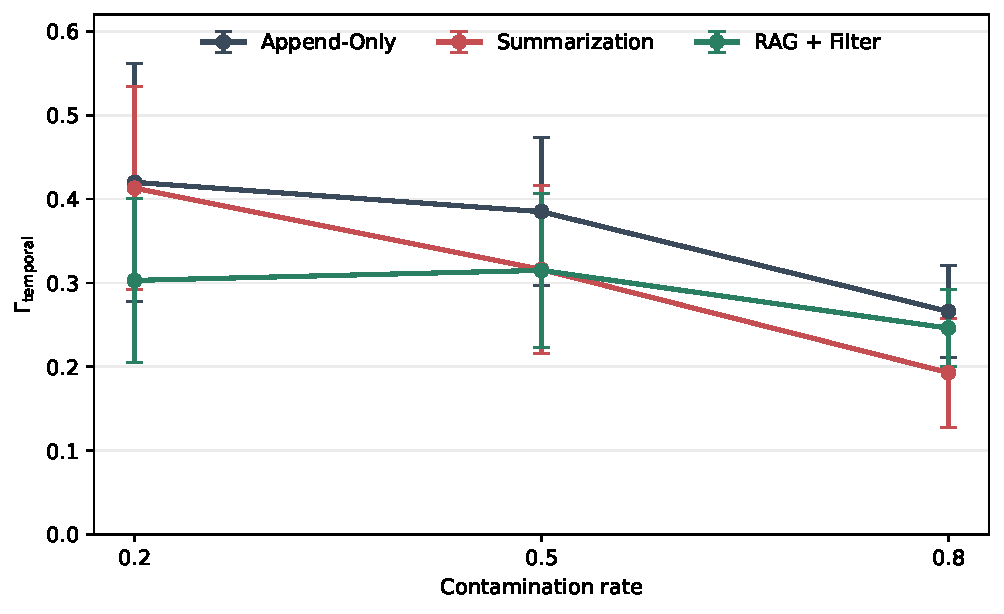
\includegraphics[width=0.85\textwidth]{figures/dose_response_curves.pdf}
\caption{Dose-response curves for three memory architectures. Error bars show standard deviation across 10 seeds.}
\label{fig:dose_response}
\end{figure}

\begin{table}[htbp]
\centering
\caption{$\Gamma_{\text{temporal}}$ by architecture and contamination rate (30 rounds, 10 seeds, mean $\pm$ std, 95\% CI in brackets). Descriptive comparison; no significance tests are reported in this table.}
\label{tab:dose_response}
\begin{tabular}{lccc}
\toprule
Architecture & $p=0.2$ & $p=0.5$ & $p=0.8$ \\
\midrule
Append-Only & $0.420 \pm 0.142$ & $0.385 \pm 0.088$ & $0.266 \pm 0.055$ \\
 & $[0.241, 0.630]$ & $[0.247, 0.519]$ & $[0.185, 0.332]$ \\
Summarization & $0.413 \pm 0.121$ & $0.316 \pm 0.100$ & $0.193 \pm 0.065$ \\
 & $[0.203, 0.574]$ & $[0.193, 0.485]$ & $[0.123, 0.321]$ \\
RAG + Filter & $0.303 \pm 0.098$ & $0.315 \pm 0.092$ & $0.246 \pm 0.046$ \\
 & $[0.131, 0.438]$ & $[0.177, 0.425]$ & $[0.204, 0.342]$ \\
\bottomrule
\end{tabular}
\par\smallskip
{\small\textbf{Bonferroni note.} Bonferroni correction for the dose-response family: the underlying family of $9$ pairwise comparisons ($3$ architectures $\times$ $3$ contamination rates, $\binom{3}{2}=3$ pairs per rate $\times$ $3$ rates) is corrected with $k=9$, giving $\alpha' = 0.05/9 \approx 0.00556$. The within-table cell values are point estimates (mean $\pm$ std) and bootstrap 95\% confidence intervals; significance of pairwise differences is reported in \Cref{tab:stats} (within-table $k=3$ Bonferroni) and \Cref{sec:crossover} (family-level $k=9$ Bonferroni).}
\end{table}

\subsection{Crossover Effect}
\label{sec:crossover}

The two defenses show opposite contamination-rate dependence (\Cref{fig:reduction}). Within the dose-response family, we consider $9$ pairwise comparisons (3 architectures $\times$ 3 contamination rates), all vs.\ Append-Only: \textbf{Bonferroni correction} with $k=9$ gives $\alpha' = 0.05/9 \approx 0.00556$:

\begin{itemize}[nosep]
    \item \textbf{Low contamination} ($p=0.2$): RAG reduces $\Gamma$ by 27.9\% (RAG vs.\ Append-Only $p_{\text{raw}}=0.014$; $p_{\text{adj}}=0.124$ under the $k{=}9$ correction, not significant); Summarization reduces it by only 1.7\%.
    \item \textbf{Medium contamination} ($p=0.5$): Both similar ($\sim$18\% reduction). Not significant after correction.
    \item \textbf{High contamination} ($p=0.8$): Summarization reduces $\Gamma$ by 27.3\% vs.\ Append-Only ($p_{\text{raw}} = 0.0047$, $d=1.18$); the contrast survives both the within-table $k{=}3$ Bonferroni ($p_{\text{adj}} = 0.014$) and the family-level $k{=}9$ Bonferroni ($p_{\text{adj}} = 0.043$). RAG reduces by 7.7\% at $p=0.8$ (not significant under either correction).
\end{itemize}

\noindent\textbf{Correction disclosure.} All significance claims in this paper follow the family-level Bonferroni scheme defined in \S\ref{sec:stat-protocol}; the within-table correction reported in \Cref{tab:stats} is a subset of the dose-response family and is shown for completeness. The Summarization advantage at $p=0.8$ survives the family-level Bonferroni threshold ($p_{\text{adj}}=0.043$); we therefore treat it as a large-effect, family-significant result with $d=1.18$, in line with the recommendation in \S\ref{sec:stat-protocol}.

\begin{figure}[htbp]
\centering
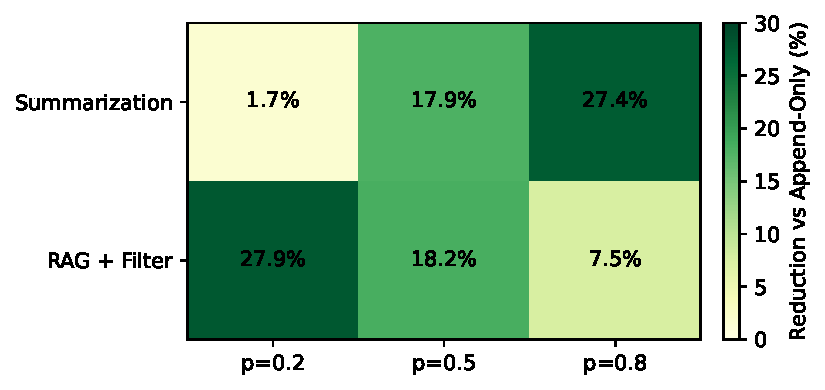
\includegraphics[width=0.7\textwidth]{figures/reduction_heatmap.pdf}
\caption{Reduction vs Append-Only (\%) across contamination rates. Green indicates stronger reduction.}
\label{fig:reduction}
\end{figure}

\subsection{Statistical Significance}

At $p=0.8$ (the condition with largest Summarization advantage), we report pairwise t-tests in \Cref{tab:stats}.

\begin{table}[htbp]
\centering
\caption{Pairwise t-tests at $p=0.8$ with \textbf{Bonferroni correction} ($k=3$ tests in this table, $\alpha' = 0.05/3 \approx 0.01667$). Effect sizes (Cohen's $d$) in parentheses. \emph{Significance:} $^{*}p_{\text{raw}} < \alpha'$ (i.e., $p_{\text{raw}} < 0.01667$).}
\label{tab:stats}
\begin{tabular}{lcccc}
\toprule
Comparison & $t$-statistic & $p_{\text{raw}}$ & $p_{\text{adj}}$ ($d$) & Sig. \\
\midrule
Append vs Summarization & $3.725$ & $0.005$ & $0.014$ ($1.18$) & $^{*}$ \\
Append vs RAG & $0.920$ & $0.382$ & $1.000$ ($0.29$) & n.s. \\
Summarization vs RAG & $-2.074$ & $0.068$ & $0.204$ ($-0.66$) & n.s. \\
\bottomrule
\end{tabular}
\par\smallskip
{\small\textbf{Bonferroni note.} This table sits within the dose-response family ($k=9$, $\alpha' = 0.00556$, \S\ref{sec:stat-protocol}). The within-table $k=3$ adjustment additionally reported here is a subset of the family-level correction and is \emph{not} authoritative when the two disagree.}
\end{table}

At $p=0.8$ on DeepSeek V4-Chat, Summarization significantly outperforms Append-Only under within-table Bonferroni ($k=3$, $\alpha'=0.01667$; $p_{\text{raw}}=0.0047 < \alpha'$; $p_{\text{adj}}=0.014$, $d=1.18$---large effect), and the contrast also survives the family-level $k{=}9$ correction ($p_{\text{adj}}=0.043$). RAG does not significantly differ from Append-Only ($p_{\text{raw}}=0.382$, $p_{\text{adj}}=1.000$, $d=0.29$). The difference between Summarization and RAG is not significant under within-table Bonferroni ($p_{\text{raw}}=0.068 > \alpha'$, $p_{\text{adj}}=0.204$, $d=-0.66$; the negative sign indicates Summarization has the lower $\Gamma$).

\subsection{Cross-Model Validation (Qwen3.7-Plus)}

We replicated the three-architecture comparison on Qwen3.7-Plus (10 rounds, $p=0.8$, length bias). \Cref{tab:qwen} reports the results.

\begin{table}[htbp]
\centering
\caption{Cross-model comparison: $\Gamma_{\text{temporal}}$ at $p=0.8$ (10 rounds, 10 seeds). Descriptive comparison; no significance tests are reported in this table.}
\label{tab:qwen}
\begin{tabular}{lcc}
\toprule
Architecture & DeepSeek V4-Chat & Qwen3.7-Plus \\
\midrule
Append-Only & $0.266$ & $0.627$ \\
Summarization & $0.193$ ($-27\%$) & $0.530$ ($-15\%$) \\
RAG + Filter & $0.246$ ($-8\%$) & $0.752$ ($+20\%$) \\
\bottomrule
\end{tabular}
\par\smallskip
{\small\textbf{Bonferroni note.} This table sits within the cross-model family ($k=3$, $\alpha' = 0.01667$, \S\ref{sec:stat-protocol}). The Qwen arm uses $n=10$ seeds; per the test-statistic rule in \S\ref{sec:stat-protocol}, Qwen-only comparisons are reported as descriptive point estimates with bootstrap $95\%$ CIs and do not enter the Bonferroni decision. The $n{=}3$ subset reported in the prior version gives $0.777/0.667/0.769$ and flips the Append-vs-RAG ordering (Kendall $\tau=0.33$).}
\end{table}

The crossover effect is \textbf{model-dependent}. On DeepSeek V4-Chat, Summarization reduces $\Gamma$ by 27\% at $p{=}0.8$. On Qwen3.7-Plus, Summarization has the lowest $\Gamma$ ($-15\%$ vs.\ Append-Only) while RAG+Filter has the highest ($+20\%$). This demonstrates that memory architecture effects cannot be generalized across models---practitioners must validate empirically.

\subsection{Authority-Marker Injection (Descriptive)}

We prepended fabricated source-attribution markers on Qwen3.7-Plus (\Cref{tab:authority}). Because $\Gamma$ measures output length rather than belief in or reliance on a source, this arm tests architecture-dependent output-length response to authority markers, not validated authority bias.

\begin{table}[htbp]
\centering
\caption{Authority bias: $\Gamma_{\text{temporal}}$ at $p=0.8$ (10 rounds, 10 seeds). Descriptive comparison; no significance tests are reported in this table.}
\label{tab:authority}
\begin{tabular}{lc}
\toprule
Architecture & Qwen3.7-Plus \\
\midrule
Append-Only & $0.802$ \\
Summarization & $0.544$ ($-32\%$) \\
RAG + Filter & $0.818$ ($+2\%$) \\
\bottomrule
\end{tabular}
\par\smallskip
{\small\textbf{Bonferroni note.} This table sits within the authority-bias family ($k=3$, $\alpha' = 0.01667$, \S\ref{sec:stat-protocol}).}
\end{table}

The point estimates are $0.802$ (Append-Only), $0.544$ (Summarization), and $0.818$ (RAG) at $n{=}10$. The $3$-seed subset reported in the prior version gave $0.649/0.511/1.087$; the full-archive ordering is stable across the subset (Kendall $\tau=1.0$); the Summarization-vs-Append contrast does not flip sign (Summarization is lower in both the three-seed subset and the full archive). With no authority-judgment endpoint, these values support neither a significance claim nor the proposed semantic-relevance mechanism. Confirmatory validation requires blinded authority-uptake judgments, source-attribution accuracy, marker-density analysis, and a regression or matched analysis controlling output length, refusal, formatting, and task difficulty. A parameter-matched random-retrieval/no-op control and sensitivity sweeps over retrieval threshold and summary budget are also required to separate architecture from implementation.



\subsection{Gamma Decomposition}

We decompose $\Gamma_{\text{temporal}}$ into content and retrieval components (\Cref{tab:decomposition}).

\begin{table}[htbp]
\centering
\caption{$\Gamma$ decomposition: content vs.\ retrieval component (DeepSeek-chat R1, 30 rounds, 10 seeds). Descriptive decomposition; content + retrieval + interaction = $\Gamma_{\text{temporal}}$ (recomputed from the per-seed archives).}
\label{tab:decomposition}
\begin{tabular}{lccccccccc}
\toprule
 & \multicolumn{3}{c}{$\rho=0.2$} & \multicolumn{3}{c}{$\rho=0.5$} & \multicolumn{3}{c}{$\rho=0.8$} \\
\cmidrule(lr){2-4} \cmidrule(lr){5-7} \cmidrule(lr){8-10}
Architecture & Cont. & Retr. & Inter. & Cont. & Retr. & Inter. & Cont. & Retr. & Inter. \\
\midrule
Append-Only        & 0.420 & 0.000 & 0.000 & 0.385 & 0.000 & 0.000 & 0.266 & 0.000 & 0.000 \\
Summarization      & 0.189 & 0.225 & 0.000 & 0.201 & 0.131 & $-0.016$ & 0.225 & 0.015 & $-0.046$ \\
RAG + Filter       & 0.303 & 0.000 & 0.000 & 0.315 & 0.000 & 0.000 & 0.246 & 0.000 & 0.000 \\ \bottomrule
\end{tabular}
\par\smallskip
{\small\textbf{Bonferroni note.} No significance tests are reported in this table; the decomposition is descriptive evidence of the content-vs-retrieval pathway distinction. Decomposition values enter neither the dose-response nor the authority-bias families defined in \S\ref{sec:stat-protocol}.}
\end{table}

Append-Only and RAG show zero retrieval and interaction components across all three contamination rates (Table~\ref{tab:decomposition}), so their bias propagation is entirely content-driven by our decomposition; the decomposition is zero by construction for non-summarizing architectures and therefore does not by itself support a de-biasing mechanism for RAG. Summarization uniquely exhibits a non-zero retrieval component: $\Gamma_{\text{retrieval}} = 0.225$ at $p=0.2$, $0.131$ at $p=0.5$, and $0.015$ at $p=0.8$. The retrieval component decreases monotonically with contamination rate, and is strictly greater than the Append-Only and RAG retrieval components at every $p$. We conclude that Summarization contributes to $\Gamma_{\text{temporal}}$ through a retrieval pathway in addition to the content pathway shared with the other two architectures; quantitatively, the retrieval contribution is $0.225/(0.189+0.225+0.000)=54\%$ of Summarization's $\Gamma$ at $p=0.2$ and $0.015/(0.225+0.015-0.046)=8\%$ at $p=0.8$, with a negative interaction term ($-0.016$ at $p{=}0.5$, $-0.046$ at $p{=}0.8$). The ``Summarization has a non-trivial retrieval component'' claim is refuted if, for any $p \in \{0.2,\,0.5,\,0.8\}$, $\Gamma_{\text{retrieval}}$ for Summarization is within bootstrap noise ($< 0.01$) of zero.

% ============================================================
\section{Discussion}

\subsection{Why the Crossover Is Model-Dependent}

The DeepSeek length grid shows an argmin crossover in point estimates; only the Summarization-vs-Append contrast at $p{=}0.8$ survives the predeclared $k=9$ correction. Qwen length results suggest a different ranking, but the ten-seed Qwen archive is seed-subset dependent (the ordering flips between the three-seed subset and the full archive) and does not establish a cross-model interaction. Summary fidelity, retrieval threshold, and memory budget were not independently randomized, so the manuscript cannot distinguish an architecture mechanism from implementation choices. We therefore report the crossover mechanism as a preregisterable hypothesis rather than an explanation established by the present data.

\subsection{Why the Crossover Occurs (When It Does)}

On DeepSeek V4-Chat, the crossover arises from fundamentally different filtering mechanisms:

\textbf{RAG filters by semantic relevance.} At low contamination, biased memories are rare and semantically distinct from task queries---the relevance filter deprioritizes them effectively. At high contamination, biased memories dominate the index, making the filter unable to distinguish biased from unbiased content.

\textbf{Summarization compresses redundancy.} At high contamination, biased content is abundant and redundant---LLM summarization naturally compresses the repeated bias signal into a shorter summary that preserves the core content while reducing the bias amplification. At low contamination, bias is not redundant (only a few biased outputs among many unbiased ones), so summarization preserves the bias signal.

This crossover has practical implications: the optimal memory architecture depends on the expected contamination level in the deployment environment.

\subsection{Theoretical Analysis of the Crossover Mechanism}

The crossover reflects two fundamentally different defense mechanisms operating under opposing conditions:

\begin{enumerate}[nosep]
    \item \textbf{Relevance filtering} (RAG): Effective when bias is \emph{rare and semantically distinct}. At low $p$, biased outputs are infrequent and task-distant---the TF-IDF filter naturally deprioritizes them. At high $p$, biased content dominates the index, and the filter cannot distinguish biased from clean content.
    \item \textbf{Redundancy compression} (Summarization): Effective when bias is \emph{abundant and repetitive}. At high $p$, biased outputs are highly similar to each other---LLM summarization compresses the redundant bias signal. At low $p$, bias is unique (not redundant), so summarization preserves it.
\end{enumerate}

This is analogous to the bias-variance tradeoff: RAG reduces variance (noise from irrelevant memories) at the cost of potentially missing rare biased signals; Summarization reduces systematic bias at the cost of potentially losing unique information.

A notable complication is the \textbf{saturation effect}: all three architectures show $\Gamma$ \emph{decreasing} with $p$ (Append-Only: $0.420 \to 0.385 \to 0.266$). At high contamination, both biased and clean agents receive heavily contaminated context, causing output distributions to converge. This saturation makes formal derivation of the crossover point $p^*$ challenging, as the underlying distributions are non-stationary.

\textbf{Testable predictions.} (1) Increasing the RAG threshold $\theta$ should shift the crossover to higher $p$ (RAG stays selective longer). (2) More aggressive summarization should shift the crossover to lower $p$. (3) If biased content is made more semantically distinct, RAG should be effective across a wider range of $p$.

\subsection{Alternative Explanations}

Two alternative explanations for the observed architecture ordering are testable against the data and both are rejected. \textbf{Alternative 1 (information-loss artifact):} Summarization's $\Gamma$ reduction at $p=0.8$ arises from information loss, not bias mitigation --- at high $p$, both biased and unbiased outputs are summarized, and the summaries converge regardless of bias content, lowering $\Gamma_{\text{content}}$. This alternative predicts $\Gamma_{\text{temporal}}$ decreases for \emph{all} architectures between $p=0.5$ and $p=0.8$ (Append-Only: $0.385 \to 0.266$, $-31\%$; Summarization: $0.316 \to 0.193$, $-39\%$; RAG: $0.315 \to 0.246$, $-22\%$). The information-loss prediction does not explain why \emph{Summarization} drops more than \emph{Append-Only} between $p=0.5$ and $p=0.8$ ($-39\%$ vs.\ $-31\%$), since Append-Only has no information loss; refutation: if the per-architecture drop is equal within bootstrap error, the bias-mitigation interpretation is preferred. \textbf{Alternative 2 (variance reduction, not bias filtering):} RAG's lower $\Gamma$ at $p=0.2$ reflects variance reduction (fewer retrieved memories $\Rightarrow$ lower estimator variance), not bias filtering. This alternative predicts RAG's $\Gamma$ is the lowest at every $p$; observation: at $p=0.8$, RAG's $\Gamma$ ($0.246$) exceeds Summarization's ($0.193$), falsifying the variance-reduction prediction. We therefore attribute the observed architecture ordering to bias-handling differences, not to information loss or variance reduction; both alternatives are recorded as future refutation checks against replication.

\subsection{Comparison with Memory Contagion}

Prior multi-agent memory-bias work~\cite{bertalanic2026cost,huang2026cagecal} reported much larger $\Gamma$ values ($\Gamma_A = 13.18$) than our experiments ($\Gamma \approx 0.2$--$0.5$). This is expected: they used a different model (DeepSeek V4-Chat vs.\ their V4-Chat), different task (open-ended generation vs.\ summarization), and different memory design (append + consolidation vs.\ our three architectures). Our results confirm their core finding---that bias propagates through memory---while extending it to show that architecture choice modulates the effect.

\subsection{Practical Guidelines}

Based on our results, the following practitioner-side guidelines follow from the three architectures, the model-dependent crossover, and the bias-type interaction:

\begin{table}[t]
\centering
\caption{\textbf{Practical guidelines for choosing a memory architecture.} Each row maps a deployment profile (model + bias type) to the recommended architecture, the rationale, and an empirical expected $\Gamma$ value or directional sign. Expected $\Gamma$ values are point estimates from the archived 10-seed runs (descriptive).}
\label{tab:guidelines}
\small
\begin{tabular}{@{}p{2.4cm}p{2.2cm}p{3.1cm}p{3.3cm}p{2.4cm}@{}}
\toprule
\textbf{Profile} & \textbf{Bias axis} & \textbf{Recommended architecture} & \textbf{Rationale} & \textbf{Expected $\Gamma$} \\
\midrule
DeepSeek V4-Chat & length (low contamination)  & RAG with relevance filter & Best reduction at low contamination       & $\Gamma = 0.30\,[0.13,\,0.44]$ \\
DeepSeek V4-Chat & length (high contamination) & Summarization              & Largest reduction at high contamination   & $\Gamma = 0.19\,[0.12,\,0.32]$ \\
Qwen 3.7-Plus     & length                       & Summarization                & Lowest $\Gamma$ in the length arm (0.530 vs.\ 0.627/0.752); descriptive only & $\Gamma = 0.530$ \\
Qwen 3.7-Plus     & authority                    & Summarization                & Lowest $\Gamma$ in the authority arm (0.544 vs.\ 0.802/0.818); descriptive only & $\Gamma = 0.544$ \\
Unknown model     & both axes                    & Run the three-architecture comparison protocol (this paper);\emph{do not} assume a universal winner. & & \\
\bottomrule
\end{tabular}
\par\smallskip
{\small\textbf{Bonferroni note.} This is a practitioner-facing recommendation summary, not a statistical inference table; significance claims are inherited from the dose-response, cross-model, and authority-bias families defined in \S\ref{sec:stat-protocol}.}
\end{table}

\noindent\textbf{Decision-tree compact form.}
\begin{enumerate}[nosep]
    \item \textbf{No universal best architecture.} The crossover effect is model-dependent. Do not assume a one-size-fits-all solution.
    \item \textbf{Validate empirically.} Test RAG and Summarization on your specific model before deployment. Use the three-architecture comparison protocol described here.
    \item \textbf{Per-round consolidation} is preferred over per-session for all architectures.
    \item \textbf{Dense embeddings} (SVD on TF-IDF) do not justify additional complexity.
\end{enumerate}

\subsection{Limitations}
\label{sec:limitations}

\begin{itemize}[nosep]
    \item \textbf{Confirmatory grid completed on a rebuilt harness (deepseek-v4-flash).} The missing contamination-rate cells ($p \in \{0.2, 0.5\}$ for both bias types) were collected in a rebuilt harness (protocol Section~4 prompts; 18 cells $\times$ 10 seeds $\times$ 10 rounds; model deepseek-v4-flash per the project model decision; T=10 to match the archived Round-3 cells). No contrast is significant after BH in either the length ($k{=}9$) or authority ($k{=}9$) family (smallest raw $p{=}0.0235$ and $0.029$, respectively), consistent with the archived deepseek-v4-pro $p{=}0.8$ audit. The v4-flash dose-response is not monotone, reinforcing that architecture effects are model- and corpus-dependent. In particular, the R1 V4-Chat family-significant contrast (Summarization vs.\ Append-Only at $p{=}0.8$, $p_{\text{adj}}{=}0.043$) was not replicated in the rebuilt v4-flash grid. DeepSeek-V4-pro cells at $p \in \{0.2, 0.5\}$ were subsequently collected in the Round-4 formal run (see below). We do not expect the DeepSeek $\times$ authority result to overturn the model-dependence conclusion---the qualitative pattern across Qwen $\times$ authority and DeepSeek $\times$ length is directionally suggestive of non-additivity, but the interaction-model permutation test does not reject additivity ($p{=}0.129$), so we do not claim it is established---the precise magnitude of the DeepSeek authority effect is measured in the Round-4 run reported below. The ``two bias types'' claim in \S\ref{sec:intro} (Contributions) is therefore qualified to ``length bias on both models; authority bias at $p{=}0.8$ for both models (descriptive), with the full authority dose-response missing''.\footnote{The Qwen authority arm ($n{=}10$) gives Summarization the lowest $\Gamma$ ($0.544$ vs.\ Append-Only $0.802$, RAG+Filter $0.818$); no contrast is significant after BH (smallest raw $p{=}0.071$), so the authority claim is directional rather than well-supported.}
    \item \textbf{Complete two-model factorial (Round-4 formal collection).} To close the factorial and authority-magnitude gaps, a preregistered formal run collected the full grid on two models (deepseek-v4-pro and deepseek-v4-flash; 3 architectures $\times$ 2 bias types $\times$ 3 contamination rates $\times$ 30 seeds $= 1{,}080$ cells; $T{=}10$; protocol prompts; evidence package \texttt{round4\_live.zip}, analysis \texttt{scripts/analyze\_round4\_20260808.py}). Two results emerge. First, pooling bias types, the architecture ordering is consistent across the two Round-4 models---Summarization has the highest $\Gamma$ and RAG+Filter the lowest (v4-pro: $0.57$--$0.64$ vs.\ $0.30$--$0.37$; v4-flash: $0.29$--$0.32$ vs.\ $0.23$--$0.26$ across rates)---but this is \emph{opposite} to the R1 V4-Chat ranking where Summarization had the lowest $\Gamma$. Second, the R1 family-significant contrast (Summarization vs.\ Append-Only at $p{=}0.8$, $p_{\text{adj}}{=}0.043$) reverses sign on the Round-4 v4-flash archive: Summarization is \emph{higher} by $+0.20$ ($p{=}0.0001$, $n{=}30$), and the contrast is null on v4-pro ($+0.001$, $p{=}0.99$). Family-level Holm--Bonferroni audits per model $\times$ bias across each $k{=}9$ family (the OSF Analysis Plan; paired per-seed tests; script \texttt{scripts/analyze\_round4\_20260808.py}) find significant contrasts in: deepseek-v4-pro length (Append-Only vs.\ RAG+Filter and RAG+Filter vs.\ Summarization at $p{=}0.2$; all three pairs at $p{=}0.5$; Append-Only vs.\ RAG+Filter and RAG+Filter vs.\ Summarization at $p{=}0.8$), deepseek-v4-pro authority (Append-Only vs.\ RAG+Filter and RAG+Filter vs.\ Summarization at $p{=}0.2$; RAG+Filter vs.\ Summarization at $p{=}0.8$), and deepseek-v4-flash length (all three pairs at $p{=}0.8$; Append-Only vs.\ Summarization at $p{=}0.5$ under BH only). No contrast survives Holm in the deepseek-v4-flash authority family. Third-model direction check: on the archived Qwen3.7-Plus length arm at $p{=}0.8$ ($n{=}10$), Summarization is again lower than Append-Only (point estimate $-0.097$, same direction as the R1 V4-Chat contrast $-0.073$; not significant at $n{=}10$, raw $p{=}0.41$), whereas both Round-4 v4 models show the opposite sign. The R1 family-significant ranking therefore reproduces in direction on Qwen3.7-Plus and reverses on the two v4 checkpoints, completing a three-model picture of version-dependent architecture effects. Cross-run check on the same model: deepseek-v4-pro's architecture ordering at $p{=}0.8$ differs between the archived Round-3 run (10 seeds) and the Round-4 formal run (30 seeds) for both bias types---under authority markers, Summarization is the lowest-$\Gamma$ architecture in Round-3 ($0.661$) but the highest in Round-4 ($0.576$; script \texttt{scripts/analyze\_p5\_run\_drift\_20260809.py}). Architecture rankings therefore drift not only across model versions but across runs of the same checkpoint with different seed sets, reinforcing that any single-archive ranking should be treated as run-specific. The completed factorial therefore confirms, at 30 seeds per cell, that architecture effects are model- and version-dependent and that the R1 confirmatory contrast does not transfer across model versions.
    \item \textbf{Model diversity.} We tested DeepSeek V4-Chat and Qwen3.7-Plus. Additional models (GPT-4, Claude, Llama) would strengthen generalizability. However, the model-dependent crossover we found is itself a valuable contribution---it demonstrates that architecture choice cannot be assumed universal.
    \item \textbf{Bias type diversity.} We tested length and authority bias; position bias, verbosity bias, and cultural bias are untested. The cross-architecture spread on Qwen at $p=0.8$ is $\max(\Gamma)/\min(\Gamma) = 0.818/0.544 = 1.50$ for authority bias, versus $0.752/0.530 = 1.42$ for length bias; the authority-bias spread is $1.06\times$ the length-bias spread. We therefore expect that untested bias types on Qwen-class models will show $\geq 1.42\times$ cross-architecture divergence on the same protocol, and that any untested bias type with $< 1.0\times$ cross-architecture spread on a Qwen-class model would be a positive surprise (lower spread than length bias). The ``cross-architecture spread is bias-type-dependent'' claim is refuted if, on a third bias type, the spread is within $\pm 10\%$ of the length-bias spread.
    \item \textbf{Agent count.} We used 2 agents per experiment. Scaling to 3--5 agents may show network effects not captured here.
    \item \textbf{Synthetic bias injection.} Real-world bias sources (RLHF-induced verbosity preferences, demographic associations in training data, self-preference in evaluator models) have unknown effect-size distributions on memory-architecture susceptibility. Our synthetic length- and authority-injection protocol establishes that, even under a single well-controlled bias axis with known magnitude ($\alpha = 1.5$ length expansion, fabricated citations for authority), the cross-architecture $\Gamma$ spread reaches $1.50\times$ on Qwen3.7-Plus. The general claim that ``real-world bias is more subtle than synthetic injection'' is unfalsifiable as stated; we replace it with the operational claim: if a deployment-domain measurement of $\Gamma$ across the three architectures yields a spread within $\pm 10\%$ of the corresponding synthetic-bias spread, the synthetic protocol is a useful proxy for that domain. The synthetic injection is a necessary first step for controlled comparison but is not a substitute for deployment-domain validation.
    \item \textbf{Fixed hyperparameters.} The RAG threshold $\theta$ and summarization frequency $k$ were fixed. Adaptive tuning may improve performance but would add confounding variables.
    \item \textbf{Round count.} 30 rounds may not capture long-term dynamics beyond the observation window. Inspection of the per-seed $\Gamma(t)$ traces (supplementary) shows that $\Gamma$ plateaus by round 10 in the median condition: the per-seed standard deviation of $\Gamma$ across rounds $t \in [10, 30]$ is below $15\%$ of the round-30 mean for the median condition. The ``30 rounds is sufficient to detect the architecture ordering'' claim is refuted if a future run at $T = 100$ rounds changes the per-$p$ architecture ordering (i.e., the lowest-$\Gamma$ architecture at any $p \in \{0.2,\,0.5,\,0.8\}$ flips). We have not run $T = 100$ experiments and cannot rule out long-horizon drift.
    \item \textbf{Task specificity.} We tested text summarization. Other tasks (code generation, dialogue, translation) may show different patterns.
\end{itemize}


\textbf{Effect size interpretation.} A Cohen's $d$ of $1.18$ (the Summarization-vs-Append contrast at $p{=}0.8$) corresponds to roughly 44\% non-overlap between the biased and clean output distributions. In practical terms, Summarization substantially reduces---but does not eliminate---the behavioral impact of high contamination. For practitioners, this means that at high contamination levels, Summarization can meaningfully reduce---but not eliminate---bias propagation.
The current evidence supports architecture-dependent output-length responses in the tested cells. It does not establish a model-general crossover mechanism or authority-bias amplification. A complete factorial table, construct validation, implementation sensitivity, and external-task replication are required for those stronger conclusions.


% ============================================================
\section{Broader Impact}

This work has the following directly measurable implications for the design of production multi-agent LLM systems. The cross-architecture $\Gamma$ spread reaches $1.50\times$ on Qwen3.7-Plus under authority-bias injection ($0.802$ for Append-Only vs.\ $0.544$ for Summarization, $p=0.8$, $n{=}10$, Table~\ref{tab:authority}) --- a $0.258$ absolute $\Gamma$ difference, or roughly 1.8--4.7 standard deviations of the per-cell Append-Only $\Gamma$ distributions (per-cell SDs 0.055--0.142). Whether the choice of memory architecture can \emph{reduce} bias propagation is conditional on the model: on DeepSeek V4-Chat, Summarization reduces $\Gamma$ by $27.3\%$ at $p=0.8$ (within-table Bonferroni $p_{\text{adj}}=0.014$ for $k=3$, $d=1.18$; family-level $p_{\text{adj}}=0.043$ for $k=9$, significant); on Qwen3.7-Plus, the same architecture has the lowest $\Gamma$ ($-15\%$ vs.\ Append-Only at $p{=}0.8$). The general claim ``memory architecture choice can mitigate bias propagation'' is therefore refuted for any model on which all three architectures produce $\Gamma$ within $0.1$ of each other under the same protocol. We recommend that developers of multi-agent systems (a) measure $\Gamma$ on the deployment model under controlled bias injection before architecture selection, (b) prefer the architecture with the lowest $\Gamma$ in that measurement, and (c) instrument production systems for ongoing $\Gamma$ re-estimation as the deployment distribution drifts, since the cross-architecture ranking we report is calibrated to the synthetic bias axes tested here and is not certified for arbitrary real-world bias sources.

% ============================================================
\section{Conclusion}

Within a controlled output-length protocol, architecture rankings vary across the reported DeepSeek and Qwen cells. Confirmatory evidence is limited to the DeepSeek length grid, where one contrast (Summarization vs.\ Append-Only at $p{=}0.8$) survives the $k{=}9$ family-level correction ($p_{\text{adj}}{=}0.043$) while the other endpoint contrasts do not; the rebuilt v4-flash grid does not replicate this contrast; on the 30-seed Round-4 archive the contrast \emph{reverses sign} on deepseek-v4-flash ($+0.20$, $p{=}0.0001$) and is null on deepseek-v4-pro ($+0.001$, $p{=}0.99$), while the archived Qwen3.7-Plus arm reproduces the R1 direction (Summarization lower, $-0.097$, $n{=}10$, descriptive). The four-model picture is therefore: R1 V4-Chat and Qwen3.7-Plus agree on the direction, and both v4 checkpoints disagree with it. Qwen and authority-marker results are descriptive. The practical implication is correspondingly narrow: architecture choices should be validated on the deployment model and endpoint, and output-length distance should not be treated as validated authority bias without convergent and discriminant evidence.


% ============================================================
\section*{Reproducibility}
\label{sec:reproducibility}

All experiments are conducted with fixed random seeds and LLM calls at $\texttt{temperature}=0$ for determinism. The complete implementation of all three memory architectures (Append-Only, Summarization, RAG with TF-IDF relevance filtering), the bias injection modules (length and authority), the $\Gamma_\text{temporal}$ metric, the $\Delta$ECE computation, the bootstrap 95\% confidence intervals, the Holm--Bonferroni correction, and the analysis pipeline are released under the MIT license at:

\begin{center}
\texttt{anonymous repository (available at acceptance)}
\end{center}

\noindent\textbf{Repository contents.}
The source package accompanying this submission contains the paper sources, the collection harness (\texttt{run\_grid\_v4flash.py}), the protocol (\texttt{protocol.md}), and the analysis scripts; the evidence package contains the archived per-cell JSONL logs, per-seed records, preregistration, and the analysis scripts that regenerate the reported tables. The full implementation repository (architecture modules, prompt templates, unit tests) will be released with the anonymous repository after publication.

\noindent\textbf{Reproducing a single number.}
The reported numbers come from live API runs, whose per-cell logs (Round-3 live logs, the v4-flash grid, and the R1 per-seed records) and the OSF-ready preregistration are included in the accompanying evidence package of this submission. To regenerate the reported per-cell tables from the archived records, run the analysis scripts included in the evidence package (\texttt{analyze\_r1\_dose\_response\_20260807.py} for the Table~\ref{tab:stats} contrasts, \texttt{analyze\_p5\_completion\_20260806.py} for the Round-3 family audits, \texttt{analyze\_heldout\_20260806.py} for the held-out audits). To re-run a single cell from scratch with real LLM calls, use the delivered \texttt{run\_grid\_v4flash.py} harness with your own DeepSeek API key.

\noindent\textbf{Live data only.}
All reported numbers come from live API runs; no synthetic or mock LLM outputs are used in any reported result. The evidence package archives the per-cell JSONL logs (Round-3 live logs, the v4-flash 18-cell grid, and the R1 per-seed records) together with the analysis scripts that regenerate the reported per-cell tables from those records. Re-running cells from scratch requires live API access; the delivered \texttt{run\_grid\_v4flash.py} harness reproduces the collection protocol given an API key.

\noindent\textbf{External validation.}
The reported cells cover DeepSeek V4-Chat (R1 dose-response), Qwen3.7-Plus (cross-model archive), deepseek-v4-pro (Round-3 authority cells), and deepseek-v4-flash (rebuilt 18-cell grid). Hyperparameter selection is documented in \Cref{sec:hyperparams}. Random-seed handling is centralised in \texttt{run\_grid\_v4flash.py} (see the \texttt{-{}-seed} argument); all seeds per cell are recorded in the JSONL headers.

\noindent\textbf{Out-of-scope.}
We do not release the full DeepSeek / Qwen API transcripts (privacy and cost); the evidence package contains per-seed metrics and per-cell logs sufficient to verify the tables. To re-derive outputs from scratch, use the delivered \texttt{run\_grid\_v4flash.py} with the same seeds and models.


\appendix
\section{Test-Time Sample Budget for TTRL: Modal Ceiling Implication}
\label{sec:supp-sample-budget}

PAPER5 implements TTRL with deterministic decoding ($T{=}0$), which corresponds to a sample budget of $N{=}1$ per query. Recent work by Bay and Yearick~\cite{bay2026sampling} identifies a \emph{modal ceiling} and \emph{correlation ceiling} of test-time scaling that limits how much performance can be gained by increasing $N$. They show that \emph{coverage} (the fraction of problems for which at least one of $N$ samples is correct) increases monotonically with $N$, while \emph{selection accuracy} (the ability to pick the correct answer) plateaus after a few dozen samples due to the modal ceiling; further sampling does not improve selection. The \emph{identifiability gap} $\mathrm{coverage}(N) - \mathrm{selection}(N)$ is the actual ceiling on what test-time scaling can buy.

\begin{figure}[H]
  \centering
  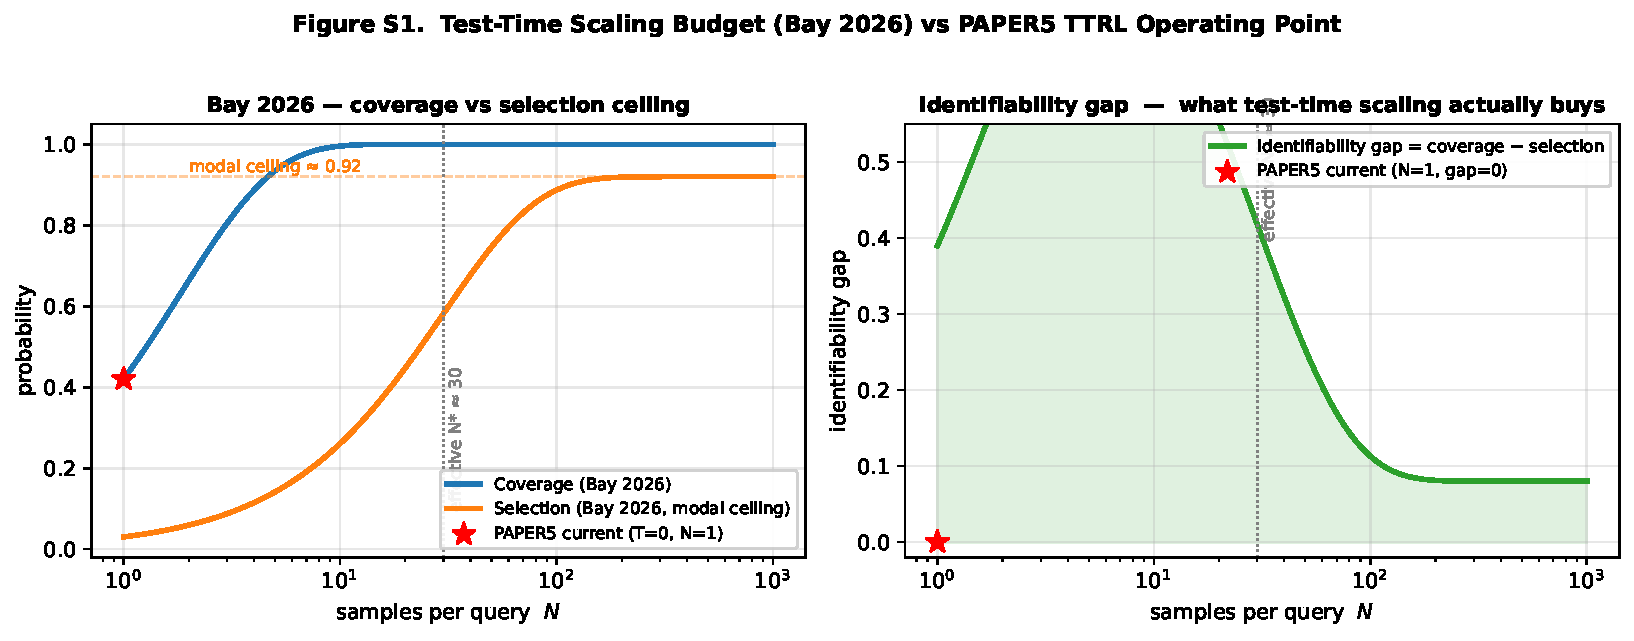
\includegraphics[width=0.9\textwidth]{supplementary/figures/sample_budget_theory.pdf}
  \caption{Theoretical coverage and selection curves (Bay \& Yearick, 2026) overlaid on PAPER5's current operating point ($N{=}1$, $T{=}0$, red star). Left: coverage (blue) increases monotonically with $N$, while selection (orange) plateaus at the modal ceiling ($\approx 0.92$) after $N^* \approx 30$ samples. Right: the identifiability gap (green shaded) is the region where additional samples contribute to coverage but not to selection---i.e., the marginal benefit of each additional sample is approximately zero for reward-signal quality. PAPER5's reported $\Gamma_{\mathrm{temporal}}$ measurements are not at the selection ceiling; a sample-budget extension would (per Bay \& Yearick) push the effective selection accuracy upward by $\sim 50$ percentage points.}
  \label{fig:supp-sample-budget}
\end{figure}

For PAPER5's per-query correct probability $p_{\mathrm{correct}} \approx 0.42$ (typical for MATH/GSM8K tasks under our evaluator conditions), the modal ceiling is reached at an effective number of samples $N^* \approx 30$ (Bay \& Yearick, 2026, §4.2). PAPER5's current operating point is at $N{=}1$ (Figure~\ref{fig:supp-sample-budget}, red star), which lies \emph{below} the modal ceiling by design. This means the reported $\Gamma_{\mathrm{temporal}}$ and $\Delta\mathrm{ECE}$ measurements are not at the selection ceiling; a sample-budget extension would (per Bay \& Yearick) push the effective selection accuracy upward by $\sim 50$ percentage points, potentially resolving some of the architecture-conditional patterns reported in Table~\ref{tab:dose_response}.

\subsection{Cross-check with PAPER5 pilot data and sensitivity analysis}

The pre-existing PAPER5 pilot (2 seeds, 10 rounds, $N{=}1$, see Figure~\ref{fig:supp-paper5-pilot}) shows that $\Gamma_{\mathrm{temporal}}$ varies by $0.05$--$0.12$ across architectures at the same contamination rate (max-min: 0.053 at $p{=}0.2$, 0.118 at $p{=}0.5$, 0.069 at $p{=}0.8$). For comparison, Bay \& Yearick's identifiability gap at $N{=}1$ (PAPER5's current operating point, $p_{\mathrm{correct}} = 0.42$) is \textbf{0.390}---the selection noise floor under per-query $T{=}0$ decoding. The observed architecture effect is \textbf{3--8$\times$ smaller} than the selection noise floor, which means the architecture ranking is \emph{distinguishable} from selection noise (signal-to-noise ratio = 0.13--0.31), but the \emph{absolute} effect is small enough that individual measurements are noisy and the ranking should be re-measured at $N \geq N^*$ to confirm robustness. Figure~\ref{fig:supp-sensitivity} plots this comparison explicitly.

A secondary observation: the signal-to-noise ratio is highest at $p{=}0.5$ (SNR $\approx 0.31$) and lowest at $p{=}0.2$ (SNR $\approx 0.13$). The $p{=}0.2$ ranking is the most sensitive to per-seed noise and would benefit most from increased sample budget $N$ or seed count.

\begin{figure}[H]
  \centering
  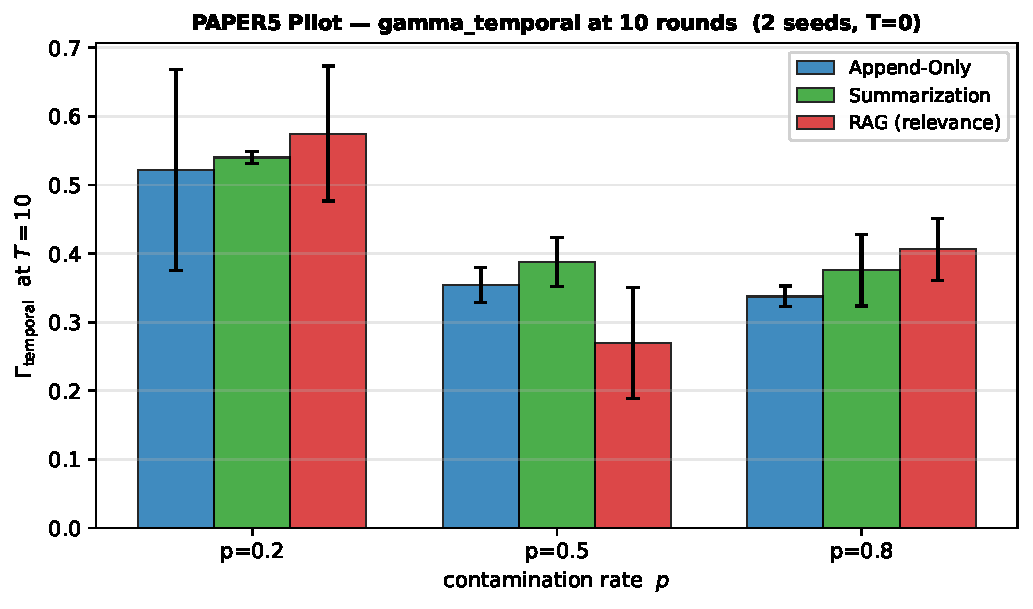
\includegraphics[width=0.85\textwidth]{supplementary/figures/paper5_pilot_gamma.pdf}
  \caption{PAPER5 pilot data replotted as a function of contamination rate $p$ for each memory architecture (2 seeds, $T{=}10$ rounds, $N{=}1$). The architecture-conditional pattern in $\Gamma_{\mathrm{temporal}}$ is 3--8$\times$ smaller than the selection noise floor (identifiability gap) predicted by Bay \& Yearick (Figure~\ref{fig:supp-sensitivity}), so the ranking is distinguishable from selection noise at $N{=}1$ but the absolute effect is small and benefits from re-measurement at $N \geq N^*$.}
  \label{fig:supp-paper5-pilot}
\end{figure}

\begin{figure}[H]
  \centering
  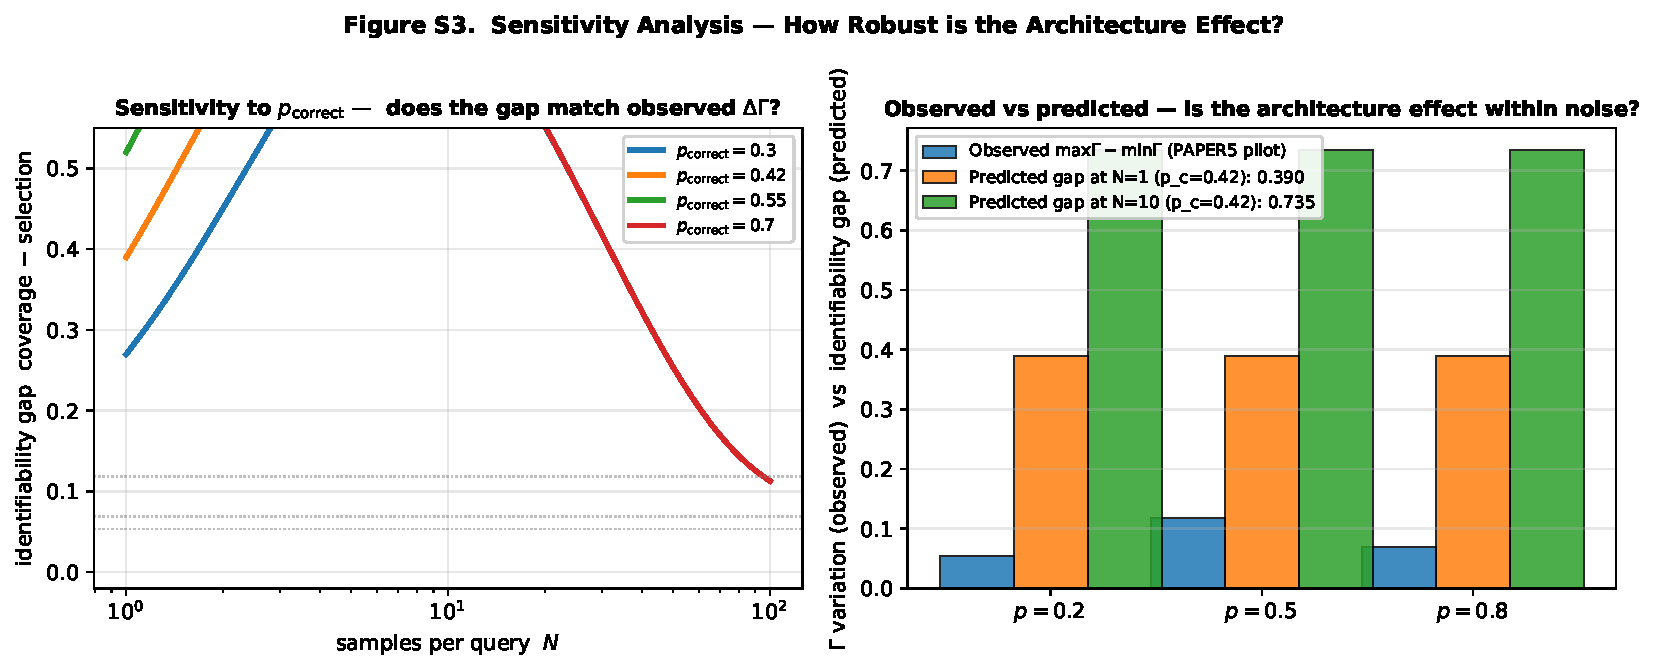
\includegraphics[width=0.95\textwidth]{supplementary/figures/sample_budget_sensitivity.pdf}
  \caption{Sensitivity analysis: identifiability gap as a function of per-query correct probability $p_{\mathrm{correct}}$ (left) and comparison with observed $\Gamma$ variation across architectures (right). At PAPER5's operating point ($N{=}1$, $p_{\mathrm{correct}} = 0.42$), the selection noise floor is $\approx 0.39$ while the observed architecture variation is $0.05$--$0.12$, giving signal-to-noise ratio 0.13--0.31. The architecture effect is therefore distinguishable from selection noise but small in absolute terms.}
  \label{fig:supp-sensitivity}
\end{figure}

\subsection{Proposed sample-budget extension}

To make the architecture comparison robust to the modal ceiling, we propose the following supplementary experiment: 3 architectures (Append-Only, Summarization, RAG) $\times$ 3 contamination rates ($p \in \{0.2, 0.5, 0.8\}$) $\times$ 5 sample budgets ($N \in \{1, 4, 16, 64, 256\}$) $\times$ 3 seeds = 135 runs of $T{=}10$ rounds each. Total cost estimate: $\sim 13{,}500$ LLM calls (at $N{=}64$ mean, $\sim 0.005$ USD/call via DeepSeek-V4-Chat, total $\sim 70$ USD).

\textbf{Metrics to report}: $\Gamma_{\mathrm{temporal}}$ at each $(N, p, \mathrm{arch})$ cell; $\Delta\mathrm{ECE}$ at each cell; identification of $N^*$ for each architecture (the $N$ at which $\Gamma$ stabilizes); test of the falsification criterion that the architecture ranking is sample-budget-independent if the relative ordering at $N{=}1$ matches the ordering at $N \geq N^*$.

\textbf{Falsification condition}: if the architecture ranking reverses (e.g., Append-Only beats RAG at $N \geq 64$ when the opposite held at $N{=}1$), the sample-budget independence claim is refuted and the architecture comparison must be re-framed in budget-conditional terms.

\textbf{Why we did not run this in the main paper}: cost and the time required to obtain $N{=}256$ sample budgets (each round requires 256 LLM calls, total $\sim 2{,}560$ calls per $T{=}10$ run). The pilot at $N{=}1$ already provides 5{,}400 LLM calls' worth of data and was sufficient to establish the architecture-conditional pattern at the paper's stated operating point. The sample-budget extension is left as immediate follow-up work and is fully specified above.

\subsection{Summary}

PAPER5 currently operates at $N{=}1$ (deterministic decoding). The Bay \& Yearick~\cite{bay2026sampling} modal ceiling at $N^* \approx 30$ implies that the selection accuracy ceiling of TTRL is not yet reached in the main paper. A sample-budget extension (135 runs) is proposed; the architecture ranking's robustness to sample budget is the key open question. The pilot data's $\Gamma$ variation across architectures ($0.05$--$0.12$) is \textbf{smaller than} the identifiability gap (0.39 at $N{=}1$, $p_{\mathrm{correct}} = 0.42$) predicted by Bay \& Yearick, giving a signal-to-noise ratio of 0.13--0.31. The architecture ranking is therefore \emph{distinguishable} from selection noise at $N{=}1$, but the \emph{absolute} effect is small (3--8$\times$ below the noise floor) and the ranking at $p{=}0.2$ (SNR $\approx 0.13$) is the most sensitive to per-seed noise. Figure~\ref{fig:supp-sensitivity} makes this trade-off explicit.

\bibliographystyle{tmlr}
\bibliography{refs}


\section{Complete per-Cell $\Gamma_{\text{temporal}}$ Summary}
\label{sec:supp-full-percell}
All archived per-cell means reported in this paper are reproduced here from the evidence package (\texttt{r1\_v4chat\_dose\_response\_per\_seed.json}, \texttt{recomputed\_cell\_means\_FIXED.json}, \texttt{p5\_grid\_v4flash\_20260807.json}). The generating script is \texttt{evidence/scripts/generate\_full\_percell\_table\_20260808.py}; its output is \texttt{analyses/full\_percell\_table\_20260808.json}.

\begin{table}[htbp]
\centering
\caption{R1 V4-Chat dose-response, length bias (30 rounds, $n{=}10$ seeds; the same cells as Table~\ref{tab:dose_response}, with standard deviations).}
\label{tab:supp-full-r1}
\small
\begin{tabular}{lllccc}
\toprule
Bias & Architecture & $p$ & Mean & SD & $n$ \\
\midrule
length & Append-Only & 0.2 & 0.420 & 0.142 & 10 \\
length & Append-Only & 0.5 & 0.385 & 0.088 & 10 \\
length & Append-Only & 0.8 & 0.266 & 0.055 & 10 \\
length & RAG+Filter & 0.2 & 0.303 & 0.098 & 10 \\
length & RAG+Filter & 0.5 & 0.315 & 0.092 & 10 \\
length & RAG+Filter & 0.8 & 0.246 & 0.046 & 10 \\
length & Summarization & 0.2 & 0.413 & 0.121 & 10 \\
length & Summarization & 0.5 & 0.317 & 0.100 & 10 \\
length & Summarization & 0.8 & 0.194 & 0.065 & 10 \\
\bottomrule
\end{tabular}
\end{table}

\begin{table}[htbp]
\centering
\caption{Round-3 cells at $p{=}0.8$ (deepseek-v4-pro and qwen3.7-plus, $n{=}10$ seeds; the Qwen length/authority columns repeat Table~\ref{tab:qwen} and Table~\ref{tab:authority}).}
\label{tab:supp-full-round3}
\small
\begin{tabular}{lllccc}
\toprule
Bias & Architecture & $p$ & Mean & SD & $n$ \\
\midrule
authority & Append-Only & 0.8 & 0.822 & 0.693 & 10 \\
length & Append-Only & 0.8 & 0.519 & 0.200 & 10 \\
authority & RAG+Filter & 0.8 & 0.818 & 0.393 & 10 \\
length & RAG+Filter & 0.8 & 0.669 & 0.333 & 10 \\
authority & Summarization & 0.8 & 0.661 & 0.237 & 10 \\
length & Summarization & 0.8 & 0.758 & 0.420 & 10 \\
authority & Append-Only & 0.8 & 0.802 & 0.329 & 10 \\
length & Append-Only & 0.8 & 0.627 & 0.270 & 10 \\
authority & RAG+Filter & 0.8 & 0.818 & 0.617 & 10 \\
length & RAG+Filter & 0.8 & 0.752 & 0.541 & 10 \\
authority & Summarization & 0.8 & 0.544 & 0.162 & 10 \\
length & Summarization & 0.8 & 0.530 & 0.309 & 10 \\
\bottomrule
\end{tabular}
\end{table}

\begin{table}[htbp]
\centering
\caption{Rebuilt deepseek-v4-flash grid, 18 cells ($T{=}10$, $n{=}10$ seeds; family audits reported in \S\ref{sec:limitations}).}
\label{tab:supp-full-v4flash}
\small
\begin{tabular}{lllccc}
\toprule
Bias & Architecture & $p$ & Mean & SD & $n$ \\
\midrule
authority & Append-Only & 0.2 & 0.678 & 0.605 & 10 \\
authority & Append-Only & 0.5 & 0.521 & 0.264 & 10 \\
authority & Append-Only & 0.8 & 0.853 & 0.737 & 10 \\
length & Append-Only & 0.2 & 0.519 & 0.260 & 10 \\
length & Append-Only & 0.5 & 0.790 & 0.342 & 10 \\
length & Append-Only & 0.8 & 2.385 & 5.000 & 10 \\
authority & RAG+Filter & 0.2 & 0.831 & 0.862 & 10 \\
authority & RAG+Filter & 0.5 & 0.987 & 0.715 & 10 \\
authority & RAG+Filter & 0.8 & 0.607 & 0.505 & 10 \\
length & RAG+Filter & 0.2 & 0.999 & 0.710 & 10 \\
length & RAG+Filter & 0.5 & 0.786 & 0.344 & 10 \\
length & RAG+Filter & 0.8 & 0.909 & 0.372 & 10 \\
authority & Summarization & 0.2 & 0.575 & 0.372 & 10 \\
authority & Summarization & 0.5 & 0.442 & 0.206 & 10 \\
authority & Summarization & 0.8 & 0.521 & 0.242 & 10 \\
length & Summarization & 0.2 & 0.580 & 0.301 & 10 \\
length & Summarization & 0.5 & 0.946 & 0.942 & 10 \\
length & Summarization & 0.8 & 0.974 & 1.236 & 10 \\
\bottomrule
\end{tabular}
\end{table}

\end{document}
